\section{Fit templates}
\label{ref:fit:tmpl}

This selection describes generation of fit templates, followed by comments on
the characteristics of the templates and configuration of fit parameters
associated with the templates.
There are a total of 37 templates in \Dz channel and 24 in \Dstar channel,
with some templates contributing to both, as listed in
\cref{tab:fit-templates-d0,tab:fit-templates-dst}.

The data-driven templates,
namely \muon misID and combinatorial background templates,
are discussed first in \cref{ref:fit:tmpl:misid,ref:fit:tmpl:comb}.

The rest are all MC templates which can be categorized into signal,
normalization, feed downs from \Dstst/heavy \Dstst/$D^{**}_s$, and contributions
from $DDX$ decay modes.
All categories share the same selection requirement as discussed in
\cref{ref:sel:mc}.
Additional global weights to account for emulation of trigger and PID
(\cref{ref:mc-emulation}),
form factor reweighting (\cref{ref:mc-cor:ff}, whenever applicable),
and corrections to detector responses (\cref{ref:mc-cor:init,ref:mc-cor:final})
are also applied according to \cref{eqn:mc-wts},
with weight-capping strategy specified:

\begin{equation}
    w_\text{tot} = \underbrace{\left(
            w_\text{trigger} \cdot w_\text{PID} \cdot
            \overbrace{
                w_\text{tracking} \cdot w_{\jpsi\kaon}
            }^\text{initial weight}
        \right)}_\text{capped at 10} \;\; \times
        \underbrace{w_\text{form factor}}_{\substack{
            \text{capped at} \\
            \text{50 for \Dz and \Dstar} \\
            \text{10 for $D^{**}$}
        }} \times \;\;
        \underbrace{
            {\textstyle\prod_i} w_\text{final weight,step $i$}
        }_\text{capped at 10}
        \label{eqn:mc-wts}
\end{equation}


% Generated in umd-lhcb/rdx-run2-analysis/fit:
%   with: make tab-fit-templates
%% D0
\begin{table}[htb]
    \caption{Fit templates included in \Dz channel fit.}
    \label{tab:fit-templates-d0}
    \footnotesize
    \centering
\begin{tabular}{lllrr}
\toprule
 {\bf Decay mode}  & {\bf Run 2 \texttt{process}} & {\bf Alias in fitter}  & {\bf Variations}  & {\bf Index} \\
\midrule
 $B^- \rightarrow D^0 \mu^- \overline{\nu}_\mu$                                       & D0Mu                     & Dmu               &            5 &       1 \\
 $\overline{B}^0 \rightarrow D^{*+} \mu^- \overline{\nu}_\mu$                         & DstMu                    & dDstmu            &           10 &       2 \\
 $B^- \rightarrow D^{*0} \mu^- \overline{\nu}_\mu$                                    & Dst0Mu                   & uDstmu            &           10 &       3 \\
 $B^- \rightarrow D^0 \tau^- \overline{\nu}_\tau$                                     & D0Tau                    & Dtau              &            5 &       4 \\
 $\overline{B}^0 \rightarrow D^{*+} \tau^- \overline{\nu}_\tau$                       & DstTau                   & dDsttau           &           10 &       5 \\
 $B^- \rightarrow D^{*0} \tau^- \overline{\nu}_\tau$                                  & Dst0Tau                  & uDsttau           &           10 &       6 \\
 $\overline{B}^0 \rightarrow D_1 \mu \overline{\nu}_\mu$                              & D1ststMu                 & dD1mu             &            3 &       7 \\
 $\overline{B}^0 \rightarrow D_1 (\rightarrow D^0 \pi\pi) \mu \overline{\nu}_\mu$     & D1ststMuD0PiPi           & dD1mu\_pipi       &            3 &       8 \\
 $\overline{B}^0 \rightarrow D^*_2 \mu \overline{\nu}_\mu$                            & D2ststMu                 & dD2mu             &            3 &       9 \\
 $\overline{B}^0 \rightarrow D'_1 \mu \overline{\nu}_\mu$                             & D1pststMu                & dD1pmu            &            2 &      10 \\
 $\overline{B}^0 \rightarrow D^*_0 \mu \overline{\nu}_\mu$                            & D0ststMu                 & dD0mu             &            2 &      11 \\
 $\overline{B} \rightarrow D^{**} (\rightarrow D^{*0} \pi\pi) \mu \overline{\nu}_\mu$ & DststHMuDst0             & Dstzpipimu        &            1 &      12 \\
 $\overline{B} \rightarrow D^{**} (\rightarrow D^* \pi\pi) \mu \overline{\nu}_\mu$    & DststHMuDst              & Dstppipimu        &            1 &      13 \\
 $\overline{B} \rightarrow D^{**} (\rightarrow D^0 \pi\pi) \mu \overline{\nu}_\mu$    & DststHMuD0               & Dpipimu           &            1 &      14 \\
 $B^- \rightarrow D_1^0 \mu \overline{\nu}_\mu$                                       & D1stst0Mu                & uD1mu             &            3 &      15 \\
 $B^- \rightarrow D_1^0 (\rightarrow D^0 \pi\pi) \mu \overline{\nu}_\mu$              & D1stst0MuD0PiPi          & uD1mu\_pipi       &            3 &      16 \\
 $B^- \rightarrow D_2^{*0} \mu \overline{\nu}_\mu$                                    & D2stst0Mu                & uD2mu             &            3 &      17 \\
 $B^- \rightarrow {D'_1}^0 \mu \overline{\nu}_\mu$                                    & D1pstst0Mu               & uD1pmu            &            2 &      18 \\
 $B^- \rightarrow {D^*_0}^0 \mu \overline{\nu}_\mu$                                   & D0stst0Mu                & uD0mu             &            2 &      19 \\
 $\overline{B}_s \rightarrow D_{s2}^* \mu \overline{\nu}_\mu$                         & Ds2Mu                    & sDs2mu            &            3 &      20 \\
 $\overline{B}_s \rightarrow D'_{s1} \mu \overline{\nu}_\mu$                          & Ds1pMu                   & sDs1pmu           &            3 &      21 \\
 $\overline{B}^0 \rightarrow D_1 \tau \overline{\nu}_\tau$                            & D1ststTau                & dD1tau            &            3 &      22 \\
 $\overline{B}^0 \rightarrow D_1 (\rightarrow D^0 \pi\pi) \tau \overline{\nu}_\tau$   & D1ststTauD0PiPi          & dD1tau\_pipi      &            3 &      23 \\
 $\overline{B}^0 \rightarrow D^*_2 \tau \overline{\nu}_\tau$                          & D2ststTau                & dD2tau            &            3 &      24 \\
 $\overline{B}^0 \rightarrow D'_1 \tau \overline{\nu}_\tau$                           & D1pststTau               & dD1ptau           &            2 &      25 \\
 $\overline{B}^0 \rightarrow D^*_0 \tau \overline{\nu}_\tau$                          & D0ststTau                & dD0tau            &            2 &      26 \\
 $B^- \rightarrow D_1^0 \tau \overline{\nu}_\tau$                                     & D1stst0Tau               & uD1tau            &            3 &      27 \\
 $B^- \rightarrow D_1^0 (\rightarrow D^0 \pi\pi) \mu \overline{\nu}_\tau$             & D1stst0TauD0PiPi         & uD1tau\_pipi      &            3 &      28 \\
 $B^- \rightarrow D_2^{*0} \tau \overline{\nu}_\tau$                                  & D2stst0Tau               & uD2tau            &            3 &      29 \\
 $B^- \rightarrow {D'_1}^0 \tau \overline{\nu}_\tau$                                  & D1pstst0Tau              & uD1ptau           &            2 &      30 \\
 $B^- \rightarrow {D^*_0}^0 \tau \overline{\nu}_\tau$                                 & D0stst0Tau               & uD0tau            &            2 &      31 \\
 $\overline{B}^0 \rightarrow D^0 D_q (\rightarrow \mu \overline{\nu}_\mu X') X$       & dDDMu                    & dDDmu             &            3 &      32 \\
 $B^- \rightarrow D^0 D_q (\rightarrow \mu \overline{\nu}_\mu X') X$                  & uDDMu                    & uDDmu             &            3 &      33 \\
 $\overline{B}^0 \rightarrow D^0 D_q (\rightarrow \tau \overline{\nu}_\tau X') X$     & dDDTau                   & dDDtau            &            0 &      34 \\
 $B^- \rightarrow D^0 D_q (\rightarrow \tau \overline{\nu}_\tau X') X$                & uDDTau                   & uDDtau            &            0 &      35 \\
 $B^-$ comb. bkg.                                                                     & BComb                    & comb              &            1 &      36 \\
 misID.                                                                               & misID                    & misID             &            1 &      37 \\
\bottomrule
\end{tabular}
\end{table}

%% Dst
\begin{table}[htb]
    \caption{Fit templates included in \Dstar channel fit.}
    \label{tab:fit-templates-dst}
    \footnotesize
    \centering
\begin{tabular}{lllrr}
\toprule
 {\bf Decay mode}  & {\bf Run 2 \texttt{process}} & {\bf Alias in fitter}  & {\bf Variations}  & {\bf Index} \\
\midrule
 $\overline{B}^0 \rightarrow D^{*+} \mu^- \overline{\nu}_\mu$                      & DstMu                    & sigmu             &           10 &       1 \\
 $\overline{B}^0 \rightarrow D^{*+} \tau^- \overline{\nu}_\tau$                    & DstTau                   & sigtau            &           10 &       2 \\
 $\overline{B}^0 \rightarrow D_1 \mu \overline{\nu}_\mu$                           & D1ststMu                 & D1                &            3 &       3 \\
 $\overline{B}^0 \rightarrow D^*_2 \mu \overline{\nu}_\mu$                         & D2ststMu                 & D2                &            3 &       4 \\
 $\overline{B}^0 \rightarrow D'_1 \mu \overline{\nu}_\mu$                          & D1pststMu                & D1p               &            2 &       5 \\
 $\overline{B} \rightarrow D^{**} (\rightarrow D^* \pi\pi) \mu \overline{\nu}_\mu$ & DststHMuDst              & D2Smu             &            1 &       6 \\
 $B^- \rightarrow D_1^0 \mu \overline{\nu}_\mu$                                    & D1stst0Mu                & uD1               &            3 &       7 \\
 $B^- \rightarrow D_2^{*0} \mu \overline{\nu}_\mu$                                 & D2stst0Mu                & uD2               &            3 &       8 \\
 $B^- \rightarrow {D'_1}^0 \mu \overline{\nu}_\mu$                                 & D1pstst0Mu               & uD1p              &            2 &       9 \\
 $\overline{B}_s \rightarrow D_{s2}^* \mu \overline{\nu}_\mu$                      & Ds2Mu                    & Ds2               &            3 &      10 \\
 $\overline{B}_s \rightarrow D'_{s1} \mu \overline{\nu}_\mu$                       & Ds1pMu                   & Ds1p              &            3 &      11 \\
 $\overline{B}^0 \rightarrow D_1 \tau \overline{\nu}_\tau$                         & D1ststTau                & D1tau             &            3 &      12 \\
 $\overline{B}^0 \rightarrow D^*_2 \tau \overline{\nu}_\tau$                       & D2ststTau                & D2tau             &            3 &      13 \\
 $\overline{B}^0 \rightarrow D'_1 \tau \overline{\nu}_\tau$                        & D1pststTau               & D1ptau            &            2 &      14 \\
 $B^- \rightarrow D_1^0 \tau \overline{\nu}_\tau$                                  & D1stst0Tau               & uD1tau            &            3 &      15 \\
 $B^- \rightarrow D_2^{*0} \tau \overline{\nu}_\tau$                               & D2stst0Tau               & uD2tau            &            3 &      16 \\
 $B^- \rightarrow {D'_1}^0 \tau \overline{\nu}_\tau$                               & D1pstst0Tau              & uD1ptau           &            2 &      17 \\
 $\overline{B}^0 \rightarrow D^* D_q (\rightarrow \mu \overline{\nu}_\mu X') X$    & dDDMu                    & dDDmu             &            3 &      18 \\
 $B^- \rightarrow D^* D_q (\rightarrow \mu \overline{\nu}_\mu X') X$               & uDDMu                    & uDDmu             &            3 &      19 \\
 $\overline{B}^0 \rightarrow D^* D_q (\rightarrow \tau \overline{\nu}_\tau X') X$  & dDDTau                   & dDDtau            &            0 &      20 \\
 $B^- \rightarrow D^* D_q (\rightarrow \tau \overline{\nu}_\tau X') X$             & uDDTau                   & uDDtau            &            0 &      21 \\
 $\overline{B}^0$ comb. bkg.                                                       & BComb                    & comb              &            1 &      22 \\
 misID.                                                                            & misID                    & misID             &            1 &      23 \\
 $D^*$ comb. bkg.                                                                  & DstComb                  & doug              &            0 &      24 \\
\bottomrule
\end{tabular}
\end{table}


\subsection{Muon misID backgrounds}
\label{ref:fit:tmpl:misid}

The \muon misID templates,
shown in \cref{fig:misid-vs-sig},
representing contributions from non-\muon tracks passing the \muon
identification requirements in ``real'' \muon samples,
are generated from the fake \muon control sample
(as in \cref{ref:sel:data:fake-mu}) with an unfolding technique.
First conceived in \cite{LHCb-ANA-2016-059}, the unfolding technique
consists of the following steps:

\begin{figure}[htb]
    \centering
    \begin{subfigure}{0.9\textwidth}
        \centering
        \caption{
            \muon misID vs. $\Bm \rightarrow \Dz\taum\neutb$ in \Dz channel.
        }
    \end{subfigure}

    \begin{subfigure}{0.9\textwidth}
        \centering
        \caption{
            \muon misID vs. $\Bzb \rightarrow \Dstarp\taum\neutb$ in \Dstar channel.
        }
    \end{subfigure}

    \caption{
        Comparison between misID and the signal templates in their
        respective channel.
    }
    \label{fig:misid-vs-sig}
\end{figure}

\begin{enumerate}
    \item Tag the fake \muon sample into $\pi$, $K$, $p$,
        $e$, and ghost\footnote{
            ``Ghost'' refers to tracks formed by random combination of hits.
        }-like species with the selection requirements listed in
        \cref{tab:selection-for-tagged-species}.
        Denote tagged species with a hat:
        $\hat{t} \in \{\hat{\pi}, \hat{K}, \hat{p}, \hat{e}, \hat{g}\}$,

    \item Obtain the efficiency for a track of true species $t$ passing \muon
        acceptance to be classified as a tagged species $\hat{t}'$
        (where $t$ and $t'$ can be the same species, e.g. a true electron
        (passing \muon acceptance) classified as a tagged electron):
        $\misEff[t]{\hat{t}'}$.
        These efficiencies are obtained from \pidcalib for $\pi, K, p, e$ and
        from MC for $g$.

    \item Given the measured yields in the fake \muon sample $\tilde{n}_{\hat{t}'}
        $ and response matrix
        $M_{\hat{t}', t^{\phantom{}}} = \misEff[t^{\phantom{}}]{\hat{t}'}$,
        % NOTE: The subscript of M is indeed tag, true!!! NOT true, tag!!!
        unfold the true yields $\tilde{n}_{t}$.
        A Bayesian unfolding (iterative unfolding) algorithm is used to obtain
        the true yields  % FIXME: citation: RooUnfold; d'Agostini's Bayesian unfolding paper
        and subsequently the efficiencies of a tagged
        $\hat{t}'$ being a true $t$: $\misEff[\hat{t}']{t}$

      \item Find $\misEff[\hat{t}']{\hat{\mu}}$,
        the transfer factor from the fake \muon sample
        (of tagged species $\hat{t}'$) to the ``real'' \muon
        samples\footnote{
            A subtlety is that here ``real'' \muon refers to the samples passing
            \muon PID cuts listed in \cref{ref:sel:data:rs}.
            Because the \muon-like particles are selected by a set of cuts,
            a hat is placed on \muon ($\hat{\mu}$!)
            to remind the reader that this sample is nothing but a \muon tag
            and is unrelated to the \muon-enriched sample (true \muon) as used
            by \pidcalib.
        },
        based on
        \begin{itemize}
            \item the efficiencies obtained in the step above,
            \item the efficiency of a track of true species $t$ that falls
                within \muon acceptance to also pass the \muon PID cuts
                $\misEff[t_\text{acc}]{\hat{\mu}}$,
            \item and the efficiency of $t_\text{acc}$ to \emph{fail} the \muon
                PID:
                $\misEff[t_\text{acc}]{t}$.
        \end{itemize}

        \begin{equation}
            \misEff[\hat{t}']{\hat{\mu}} =
                \sum_{t}
                \frac{\misEff[\hat{t}']{t}}{\misEff[t_\text{acc}]{t}}
                \misEff[t_\text{acc}]{\hat{\mu}}
        \end{equation}
        The last two efficiencies are found from \pidcalib.

    \item Apply $\misEff[\hat{t}']{\hat{\mu}}$ as a weight for each
        tagged species $\hat{t}'$ in the fake \muon sample.
        The weighted yield of tagged species $\hat{t}$ represents the \muon misID
        contributions of $\hat{t}$ to the ``real'' \muon samples.
\end{enumerate}

Comparisons between tagged and unfolded (true) yields of the fake \muon sample
are shown in \cref{fig:unfolding-binning-vars}.
The weighted yields are projected in fit variables with finer binning;
these are shown in \cref{fig:unfolding-fit-vars}.
Some of the efficiencies obtained with \pidcalib are negative; these are shifted
back to a value between $[0, 1]$ with a procedure described in
\cref{appx:formal:shift-neg-eff}.
A more detailed description of the unfolding procedure is documented in
\cref{appx:unfold-tech}.

% Generated in /misid-unfolding, with the command
%   make plot-rdx-bin_vars-ana-2016
\begin{figure}[htb]
    \centering
    \begin{subfigure}[b]{0.32\textwidth}
        \centering
        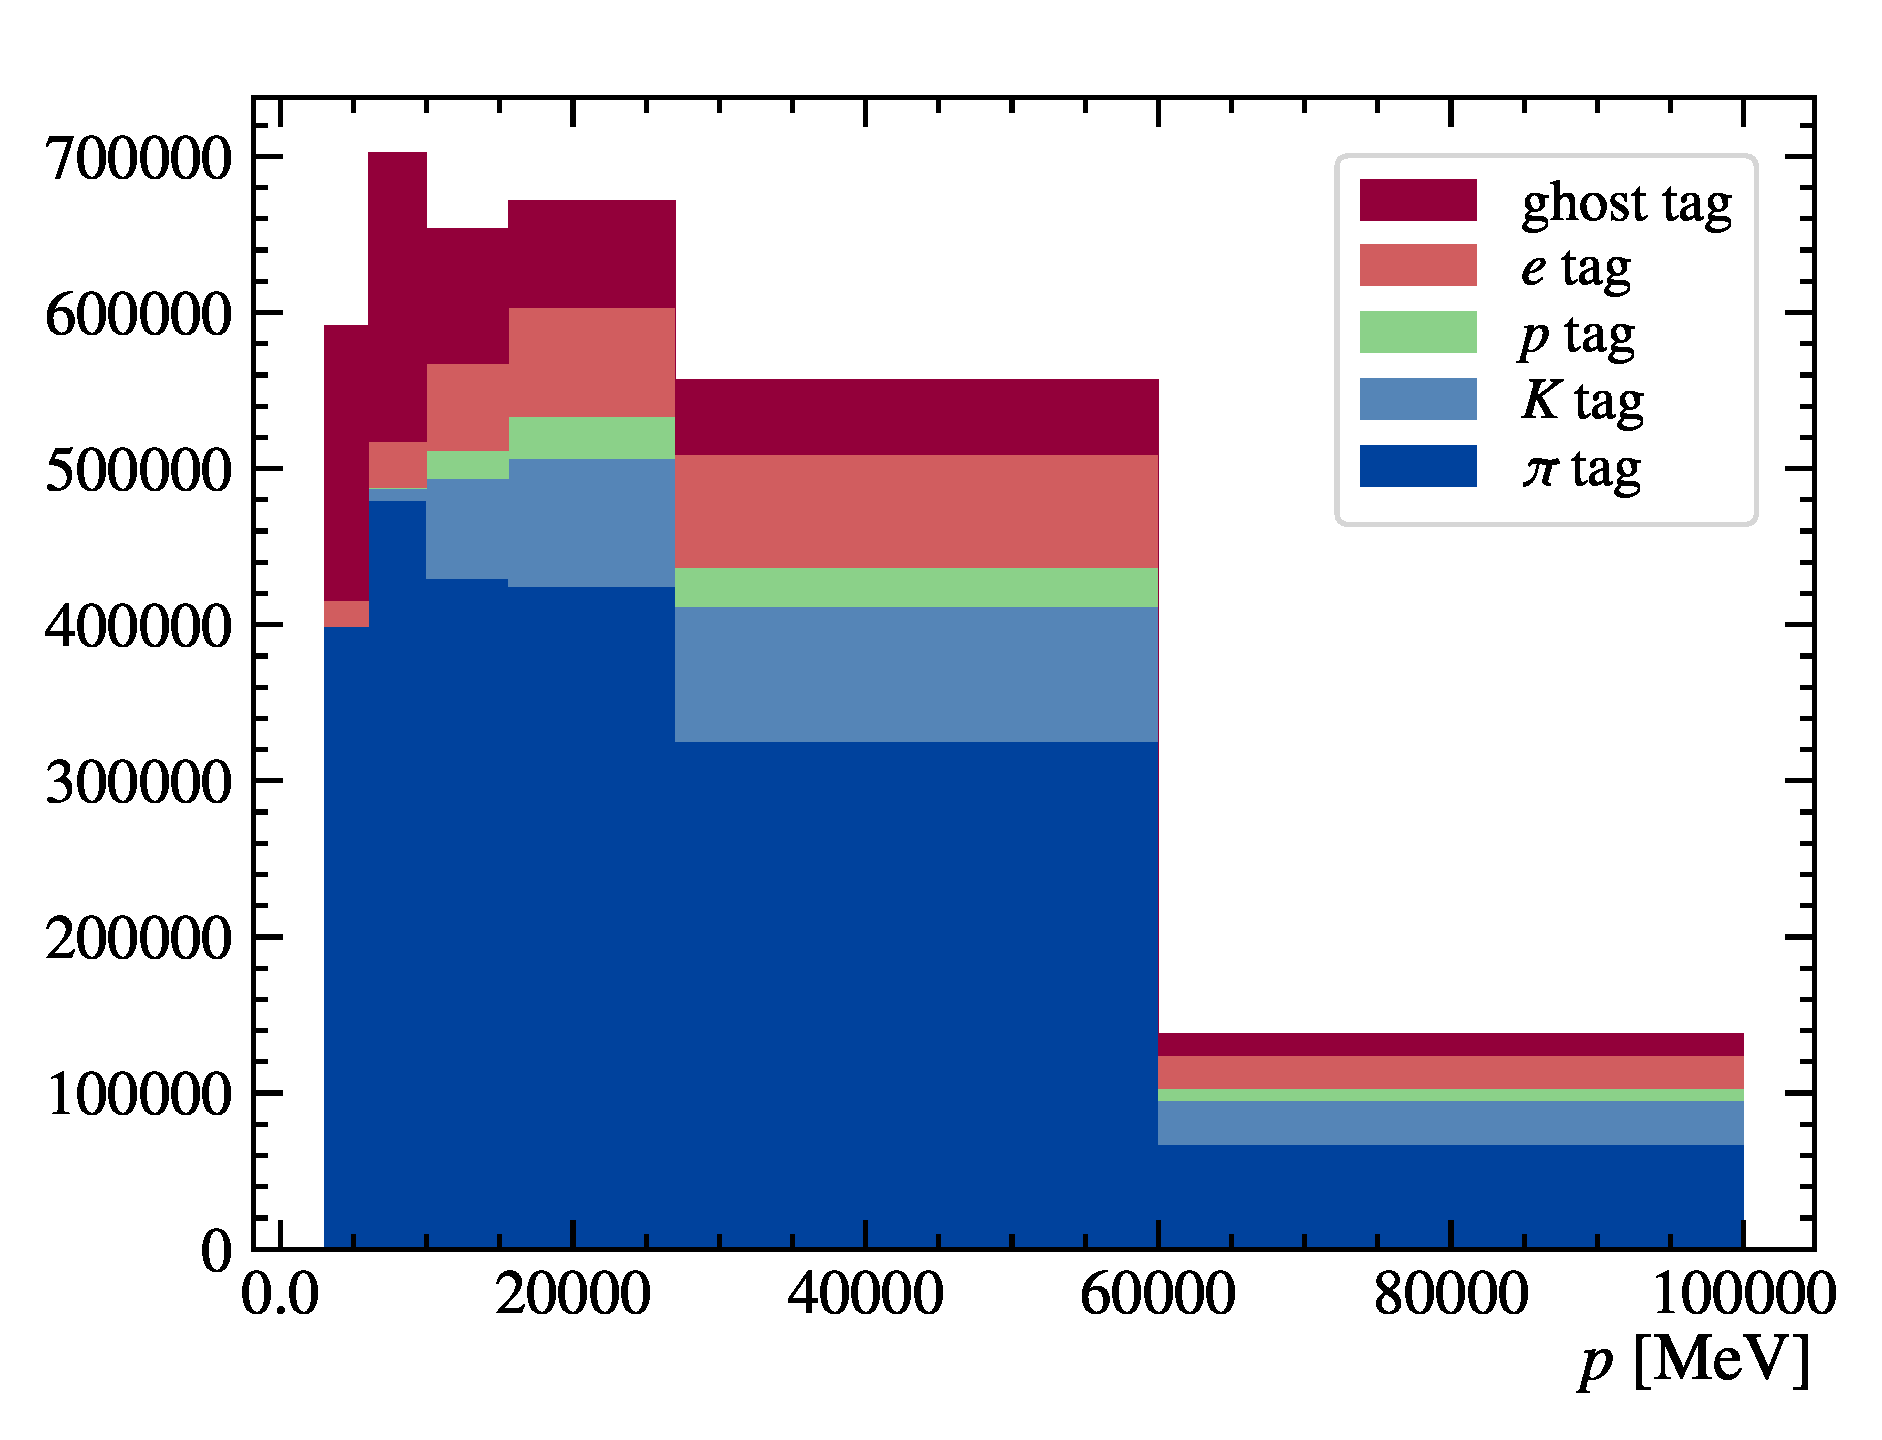
\includegraphics[width=\textwidth]{figs-fit-fit-templates/data-driven-plots/misid/D0-tag_p.pdf}
    \end{subfigure}
    \hfill
    \begin{subfigure}[b]{0.32\textwidth}
        \centering
        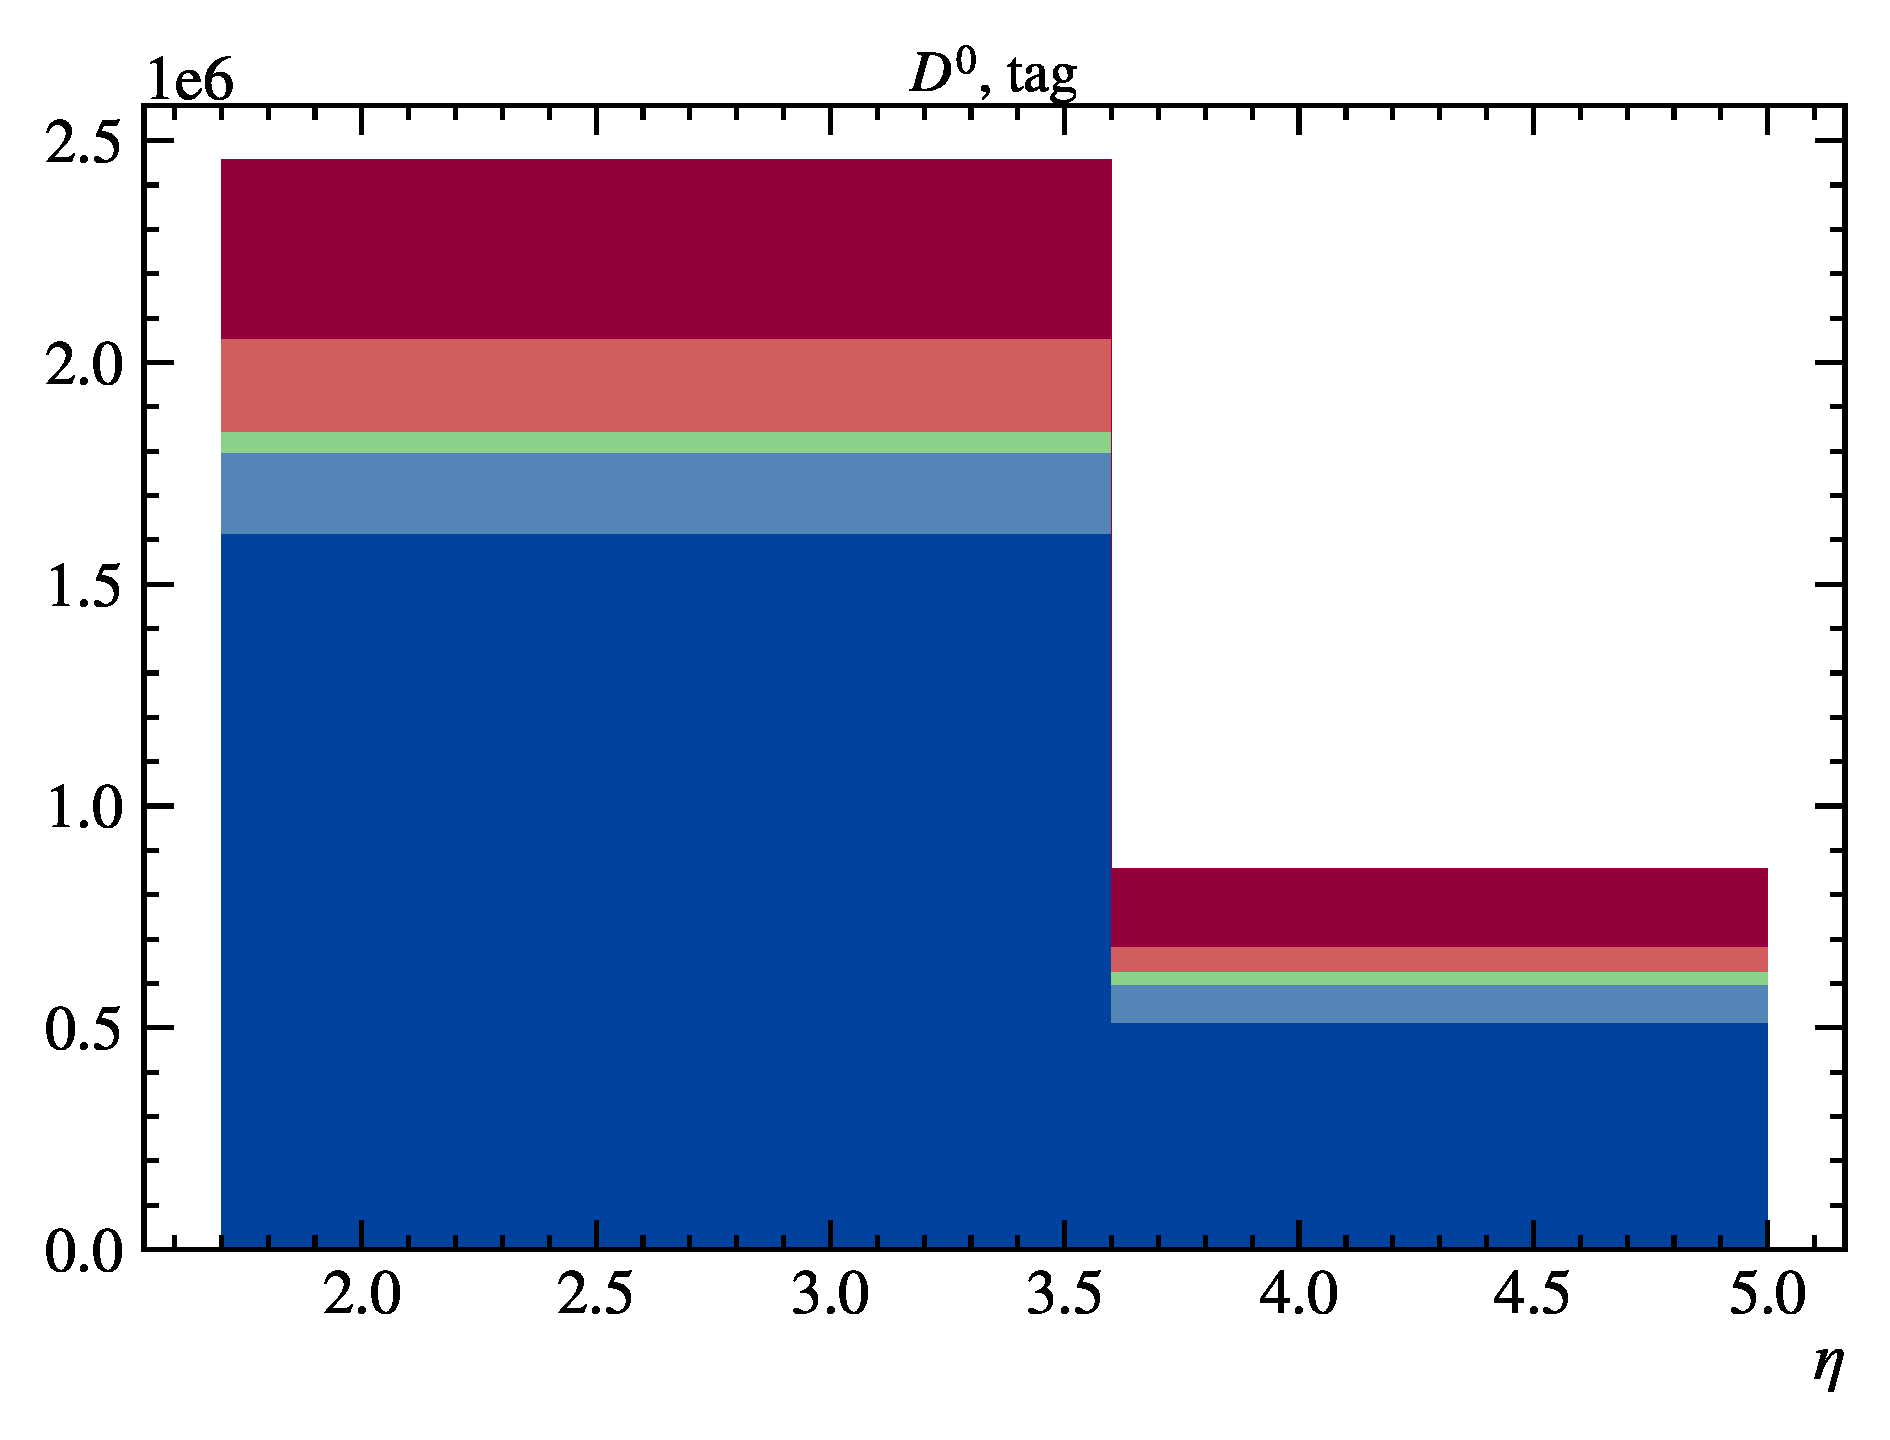
\includegraphics[width=\textwidth]{figs-fit-fit-templates/data-driven-plots/misid/D0-tag_eta.pdf}
    \end{subfigure}
    \hfill
    \begin{subfigure}[b]{0.32\textwidth}
        \centering
        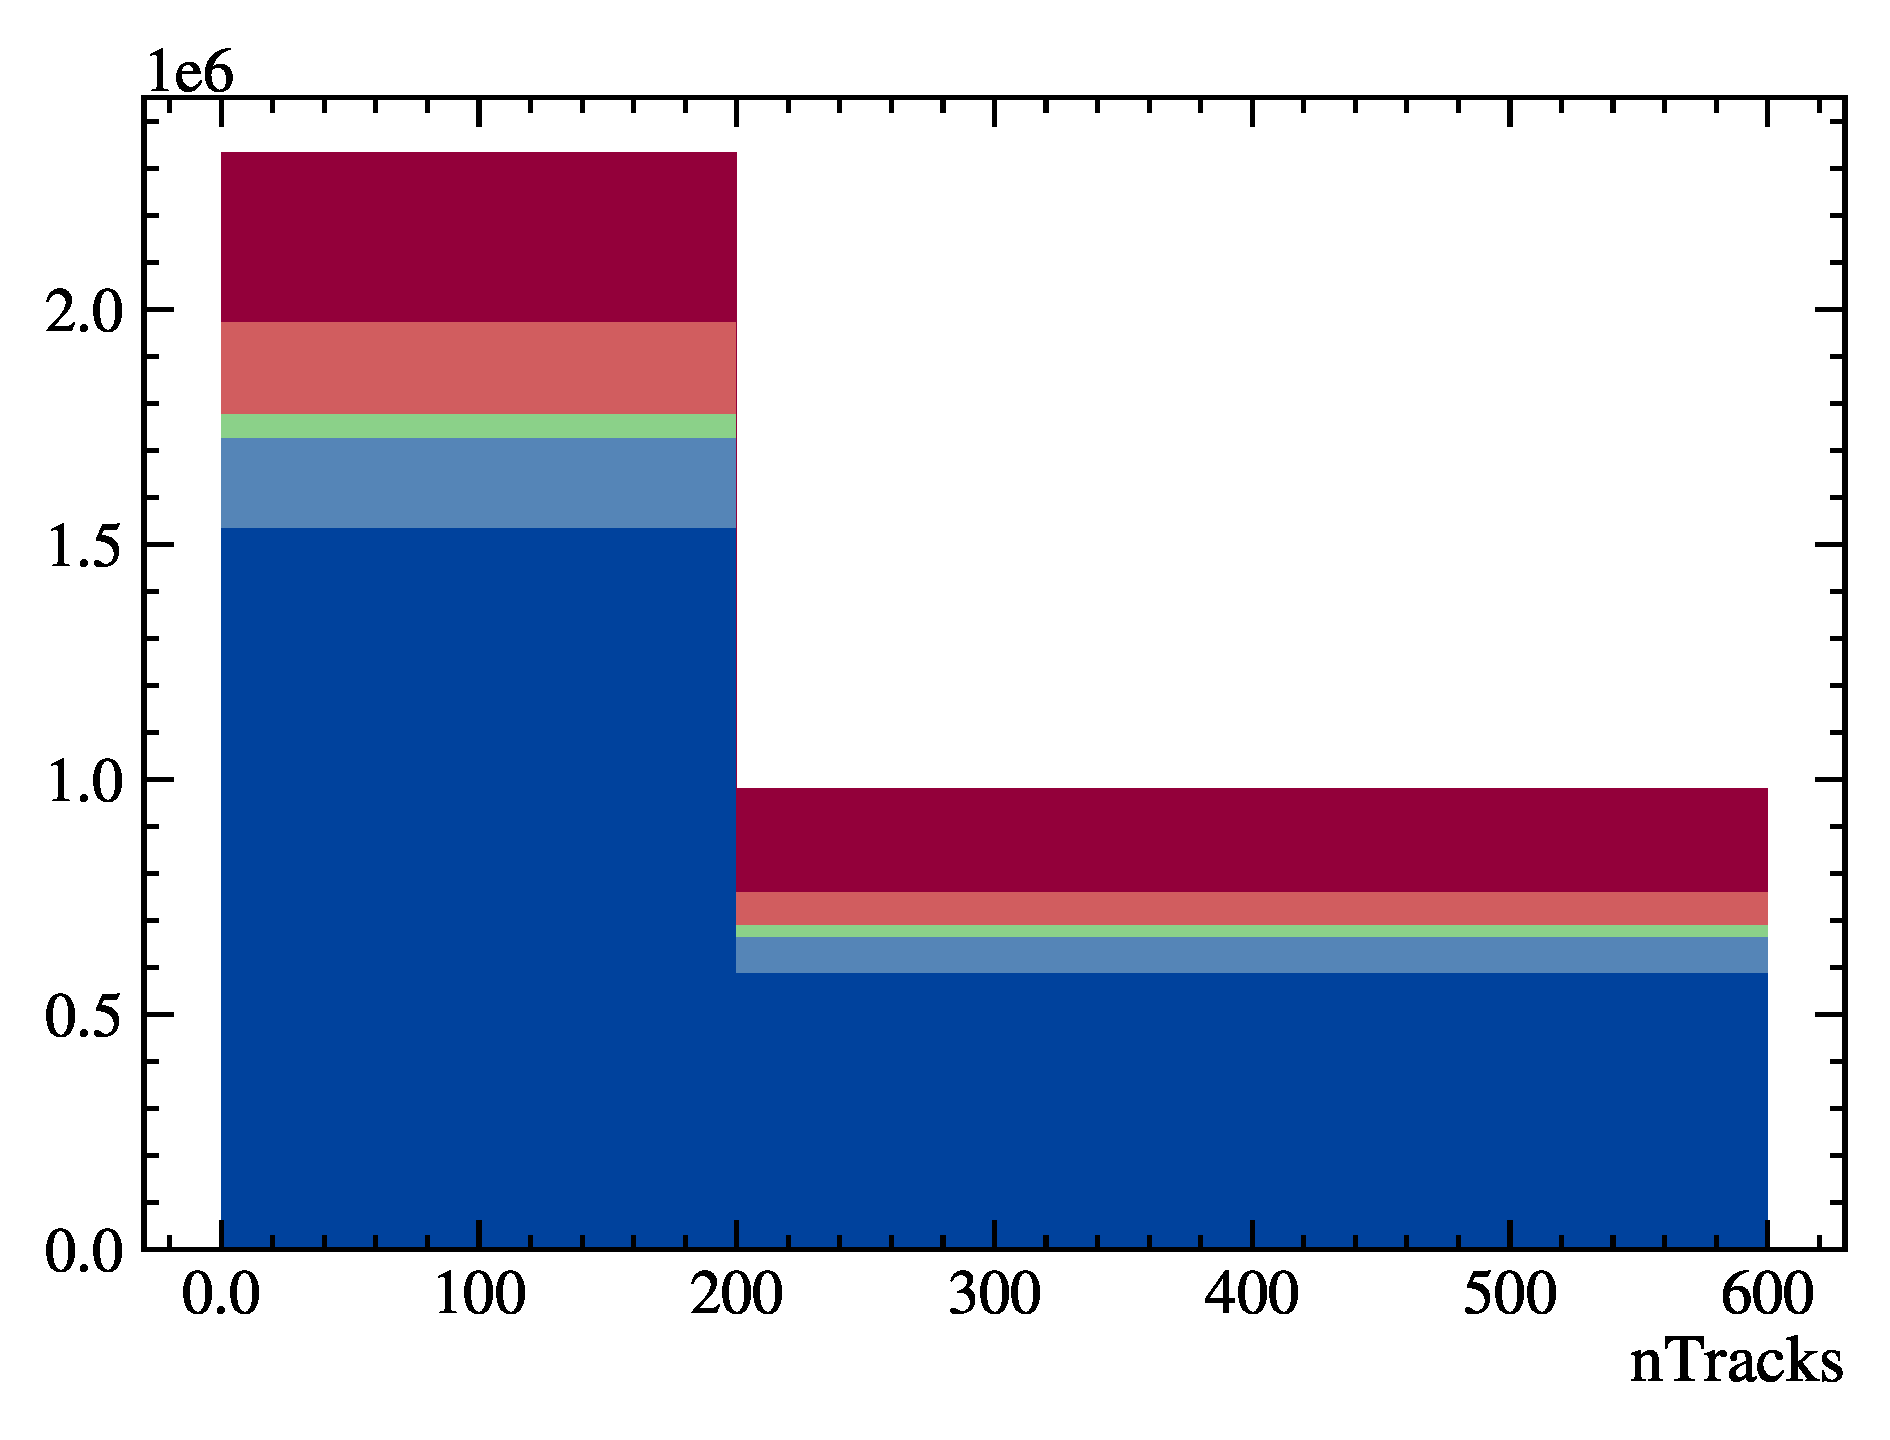
\includegraphics[width=\textwidth]{figs-fit-fit-templates/data-driven-plots/misid/D0-tag_ntracks.pdf}
    \end{subfigure}
    \\
    \begin{subfigure}[b]{0.32\textwidth}
        \centering
        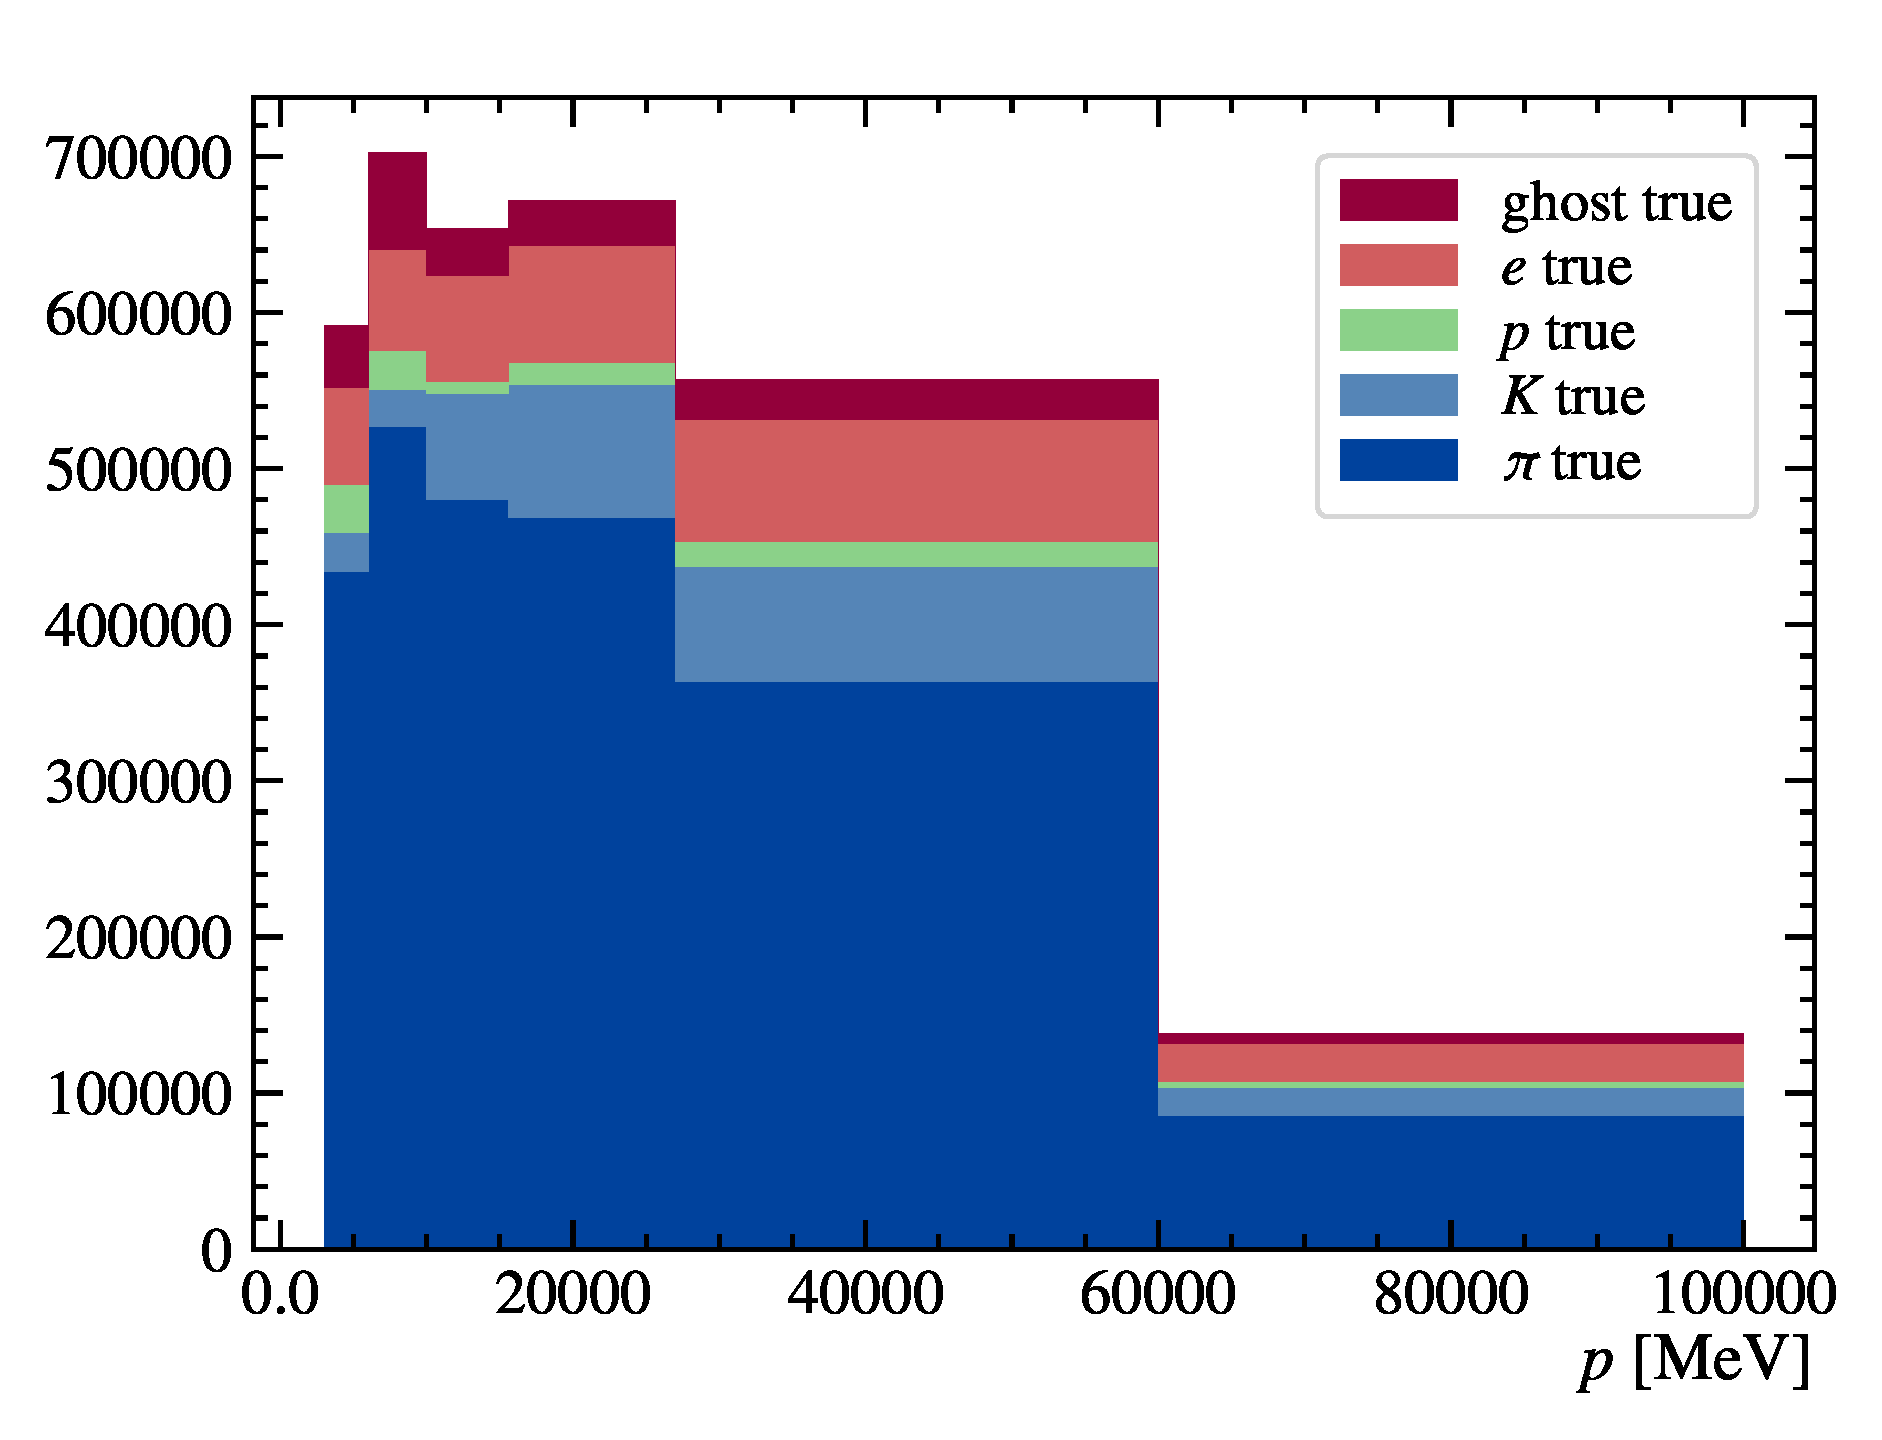
\includegraphics[width=\textwidth]{figs-fit-fit-templates/data-driven-plots/misid/D0-true_p.pdf}
    \end{subfigure}
    \hfill
    \begin{subfigure}[b]{0.32\textwidth}
        \centering
        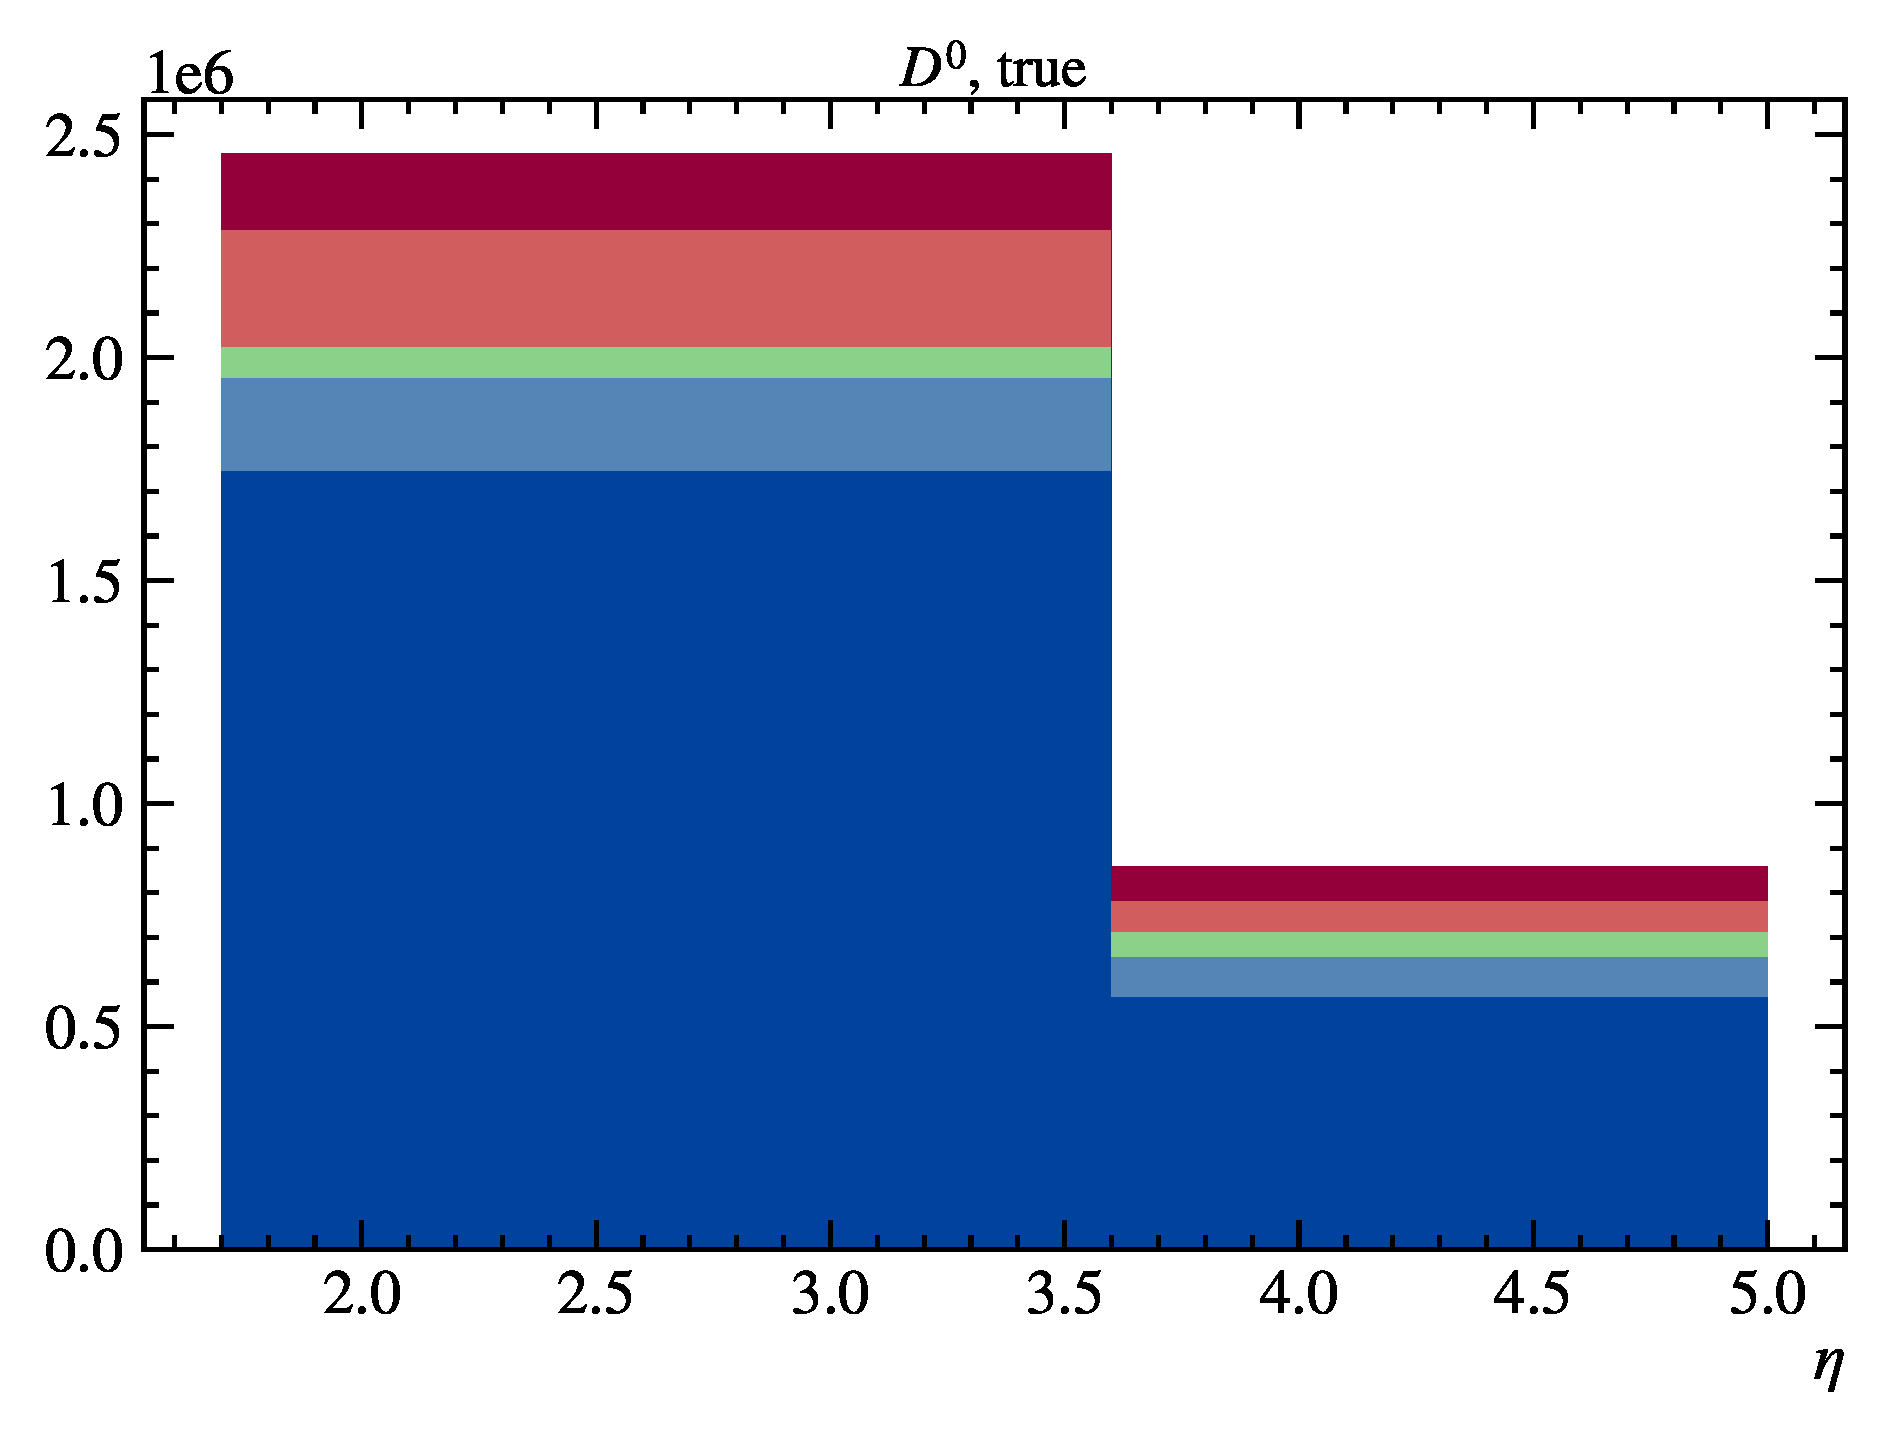
\includegraphics[width=\textwidth]{figs-fit-fit-templates/data-driven-plots/misid/D0-true_eta.pdf}
    \end{subfigure}
    \hfill
    \begin{subfigure}[b]{0.32\textwidth}
        \centering
        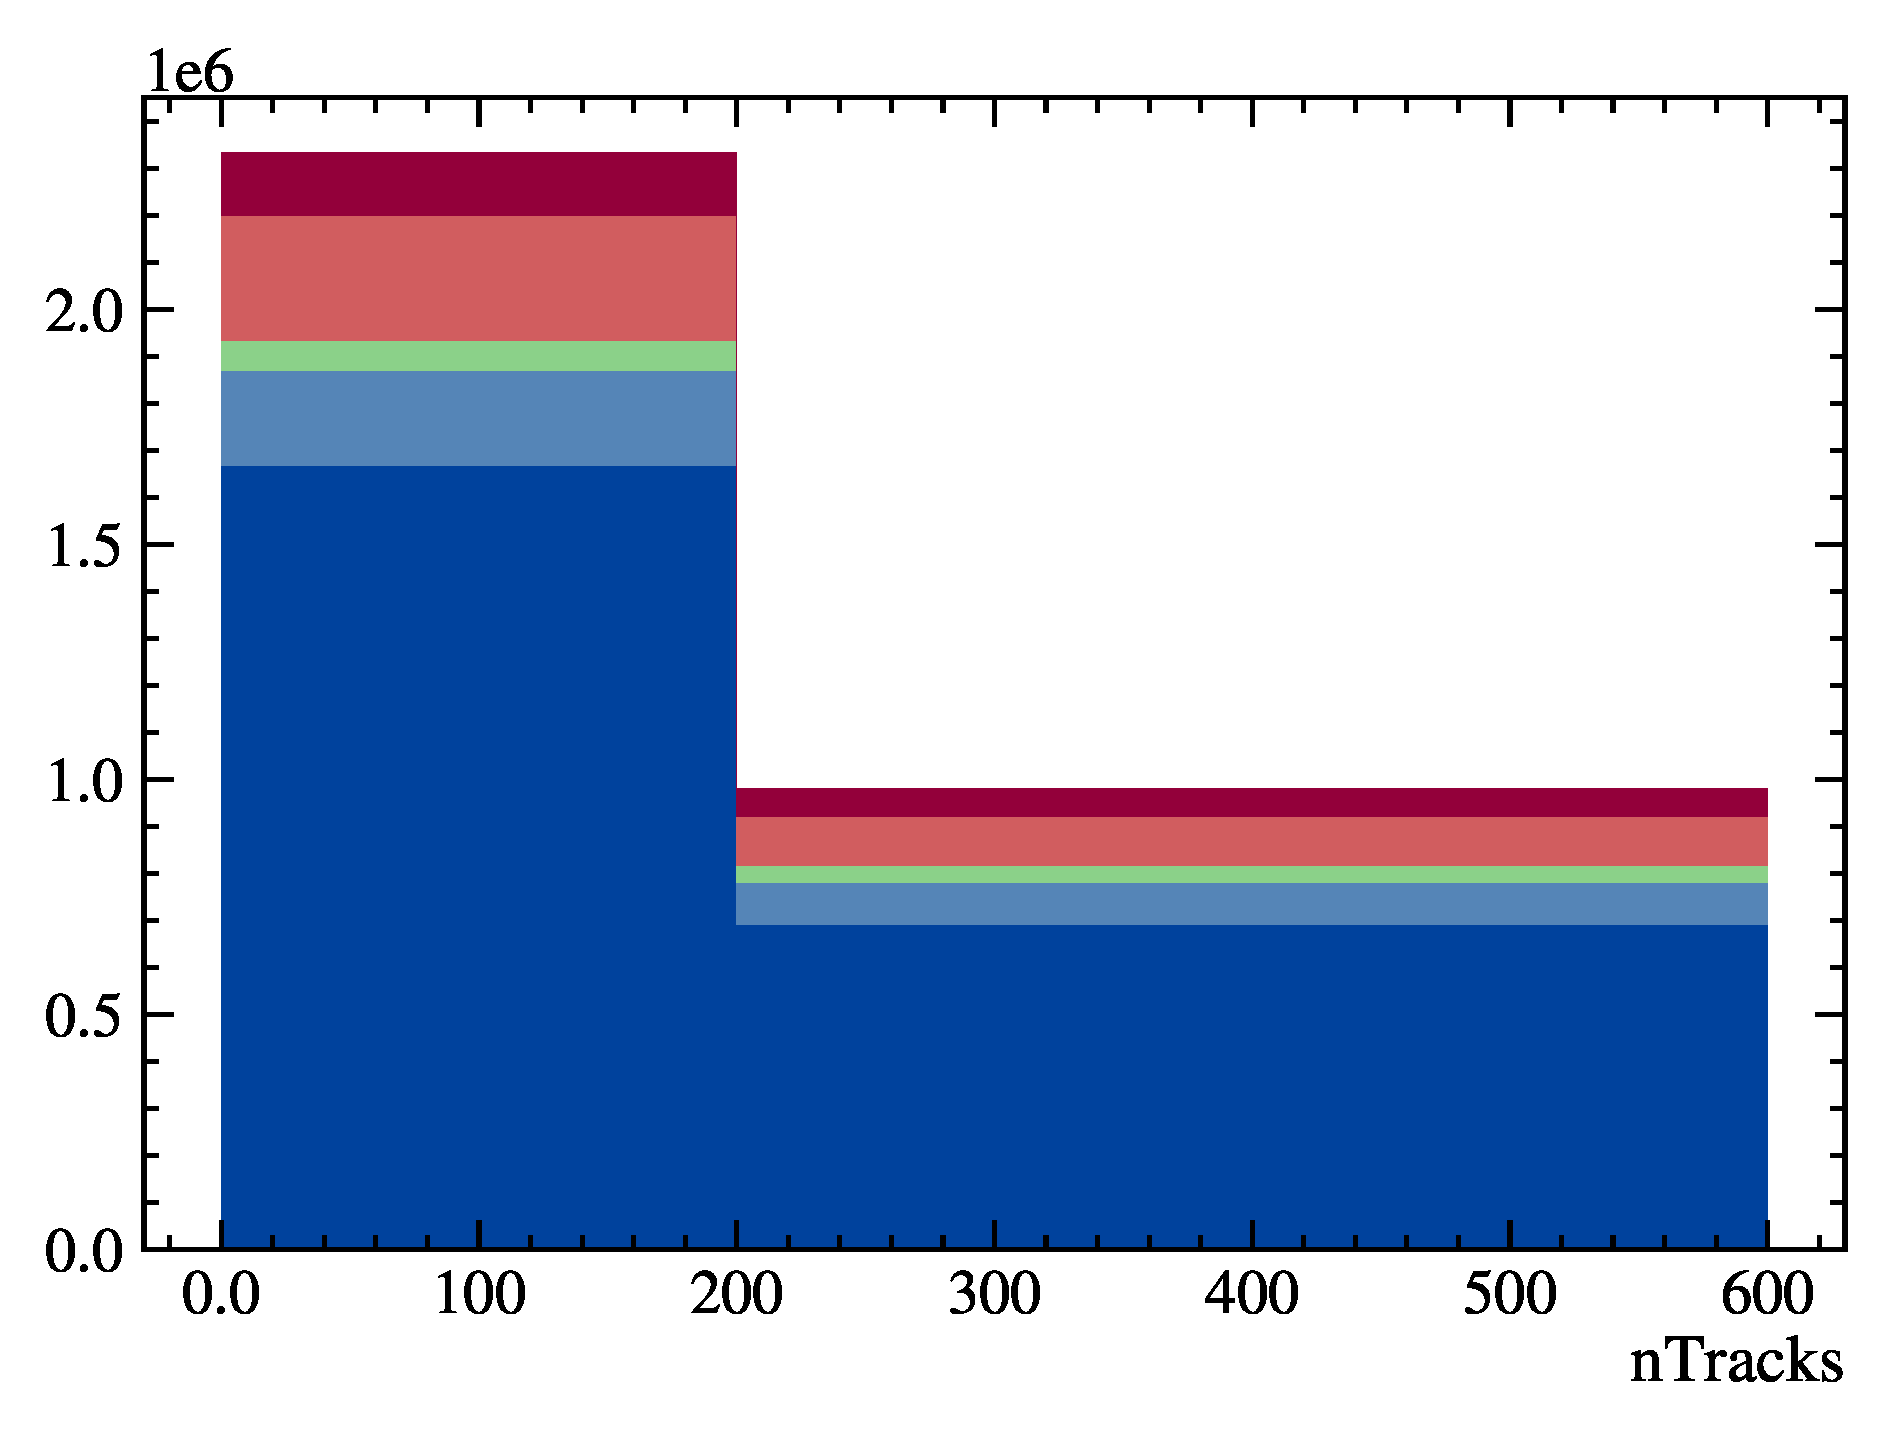
\includegraphics[width=\textwidth]{figs-fit-fit-templates/data-driven-plots/misid/D0-true_ntracks.pdf}
    \end{subfigure}
    \caption[misID tagged vs. unfolded.]{
        Unfolding effect displayed in $p$ and $\eta$ of the fake $\mu$ track,
        and nTracks of the reconstructed event.
        Top are the raw tagged yields,
        bottom are the unfolded true yields.
        The number of events is conserved by unfolding.

        The samples displayed here are 2016 $D^0$ fake \muon control samples
        $B^- \rightarrow D^0 t^-$ passing selections listed in
        \cref{ref:sel:data:fake-mu}.
    }
    \label{fig:unfolding-binning-vars}
\end{figure}

% Generated in /lhcb-ntuples-gen/studies/plot-RDX_misid_unfold_fit_vars, by
% running the script gen.sh inside
\begin{figure}[htb]
    \centering
    \begin{subfigure}[b]{0.32\textwidth}
        \centering
        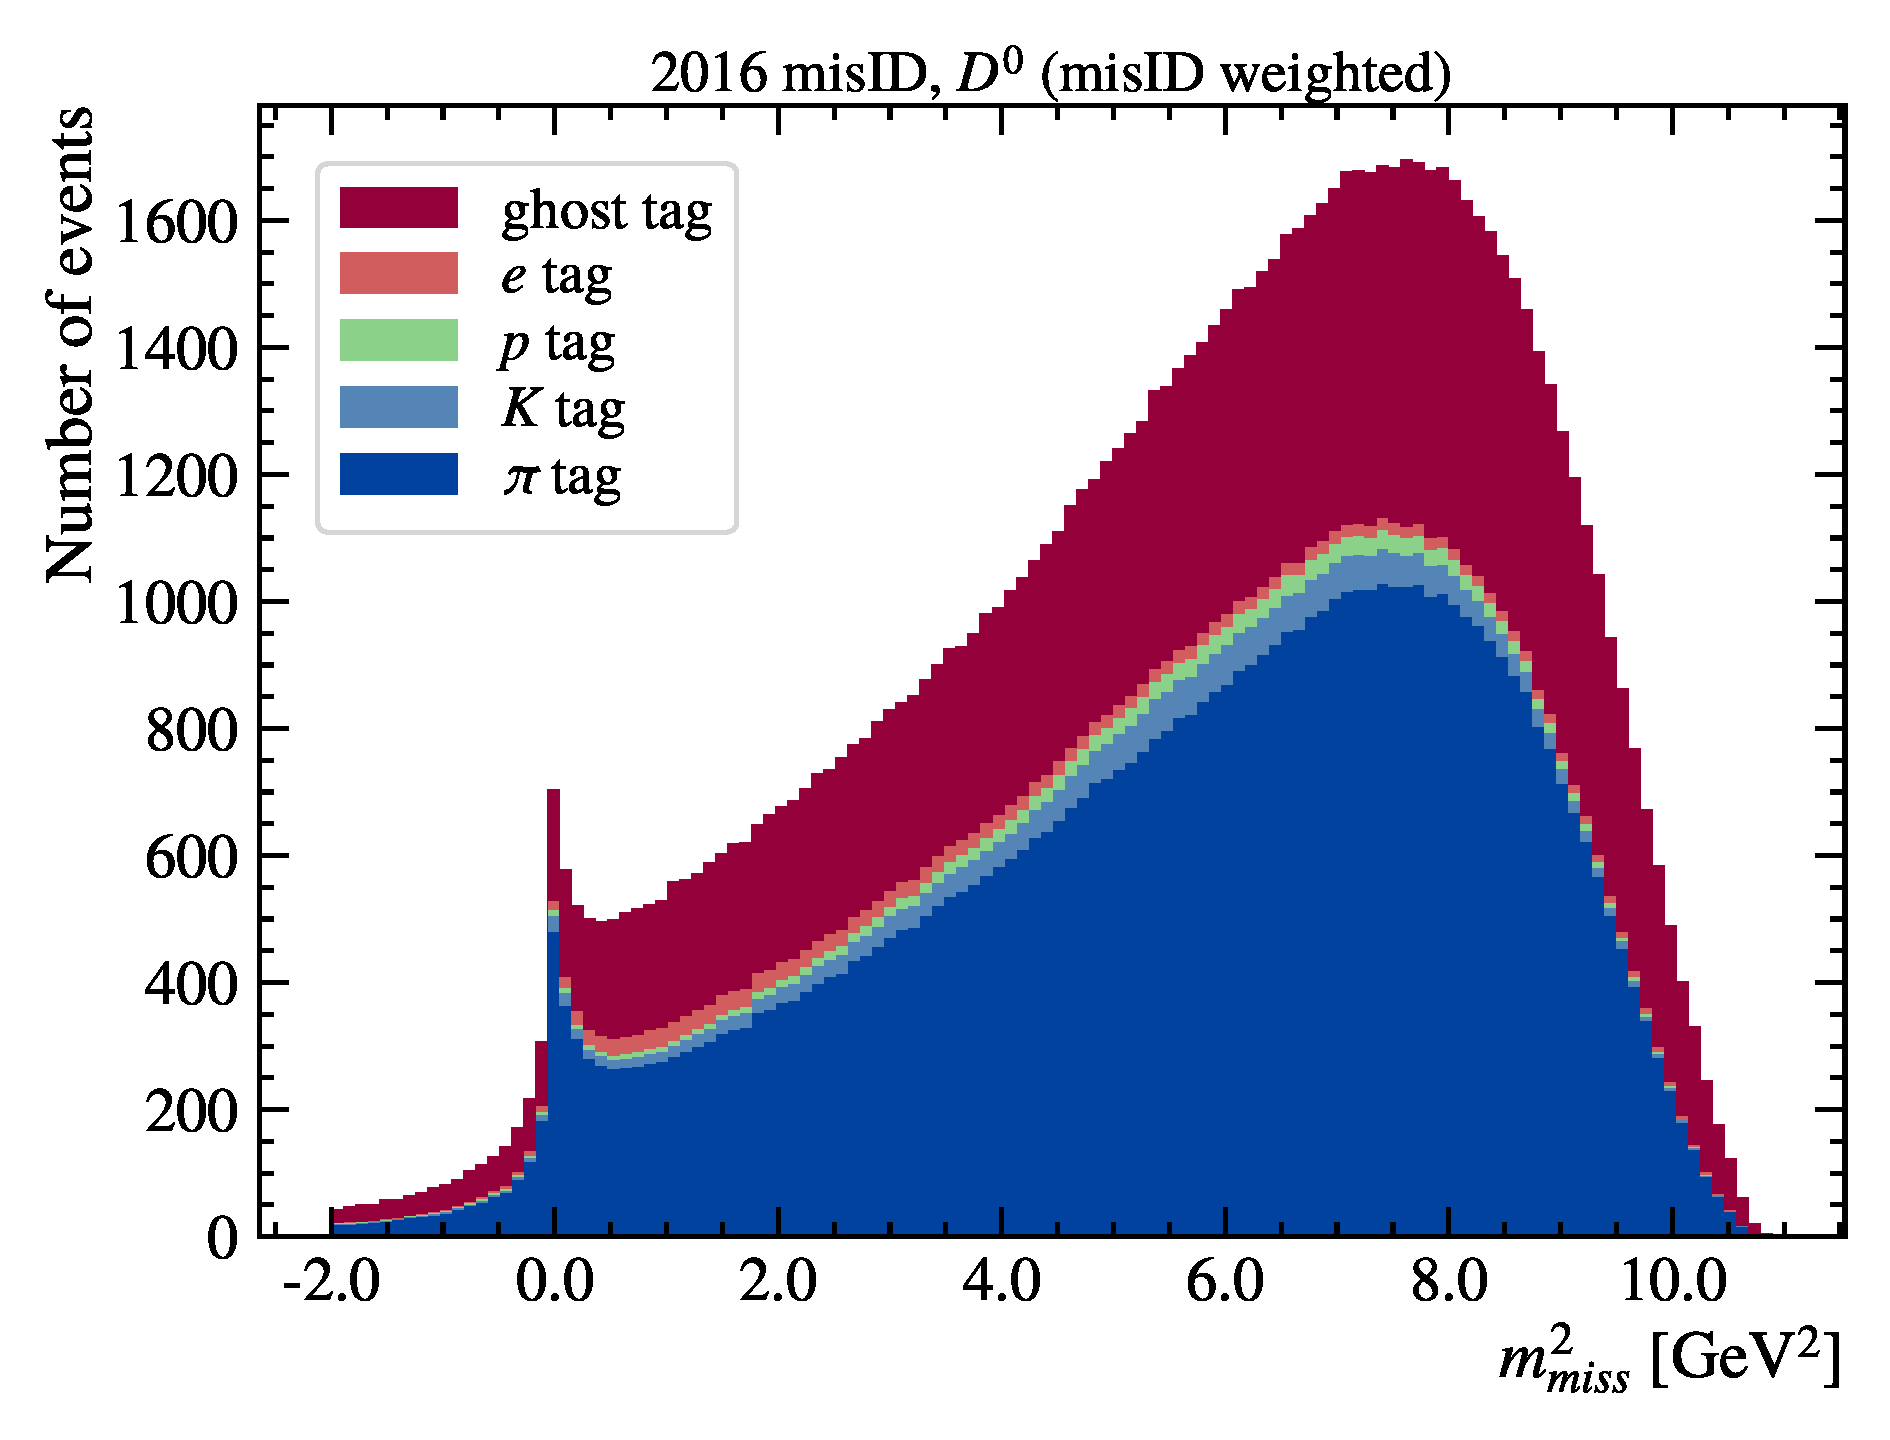
\includegraphics[width=\textwidth]{figs-fit-fit-templates/data-driven-plots/misid/D0_mm2.pdf}
    \end{subfigure}
    \hfill
    \begin{subfigure}[b]{0.32\textwidth}
        \centering
        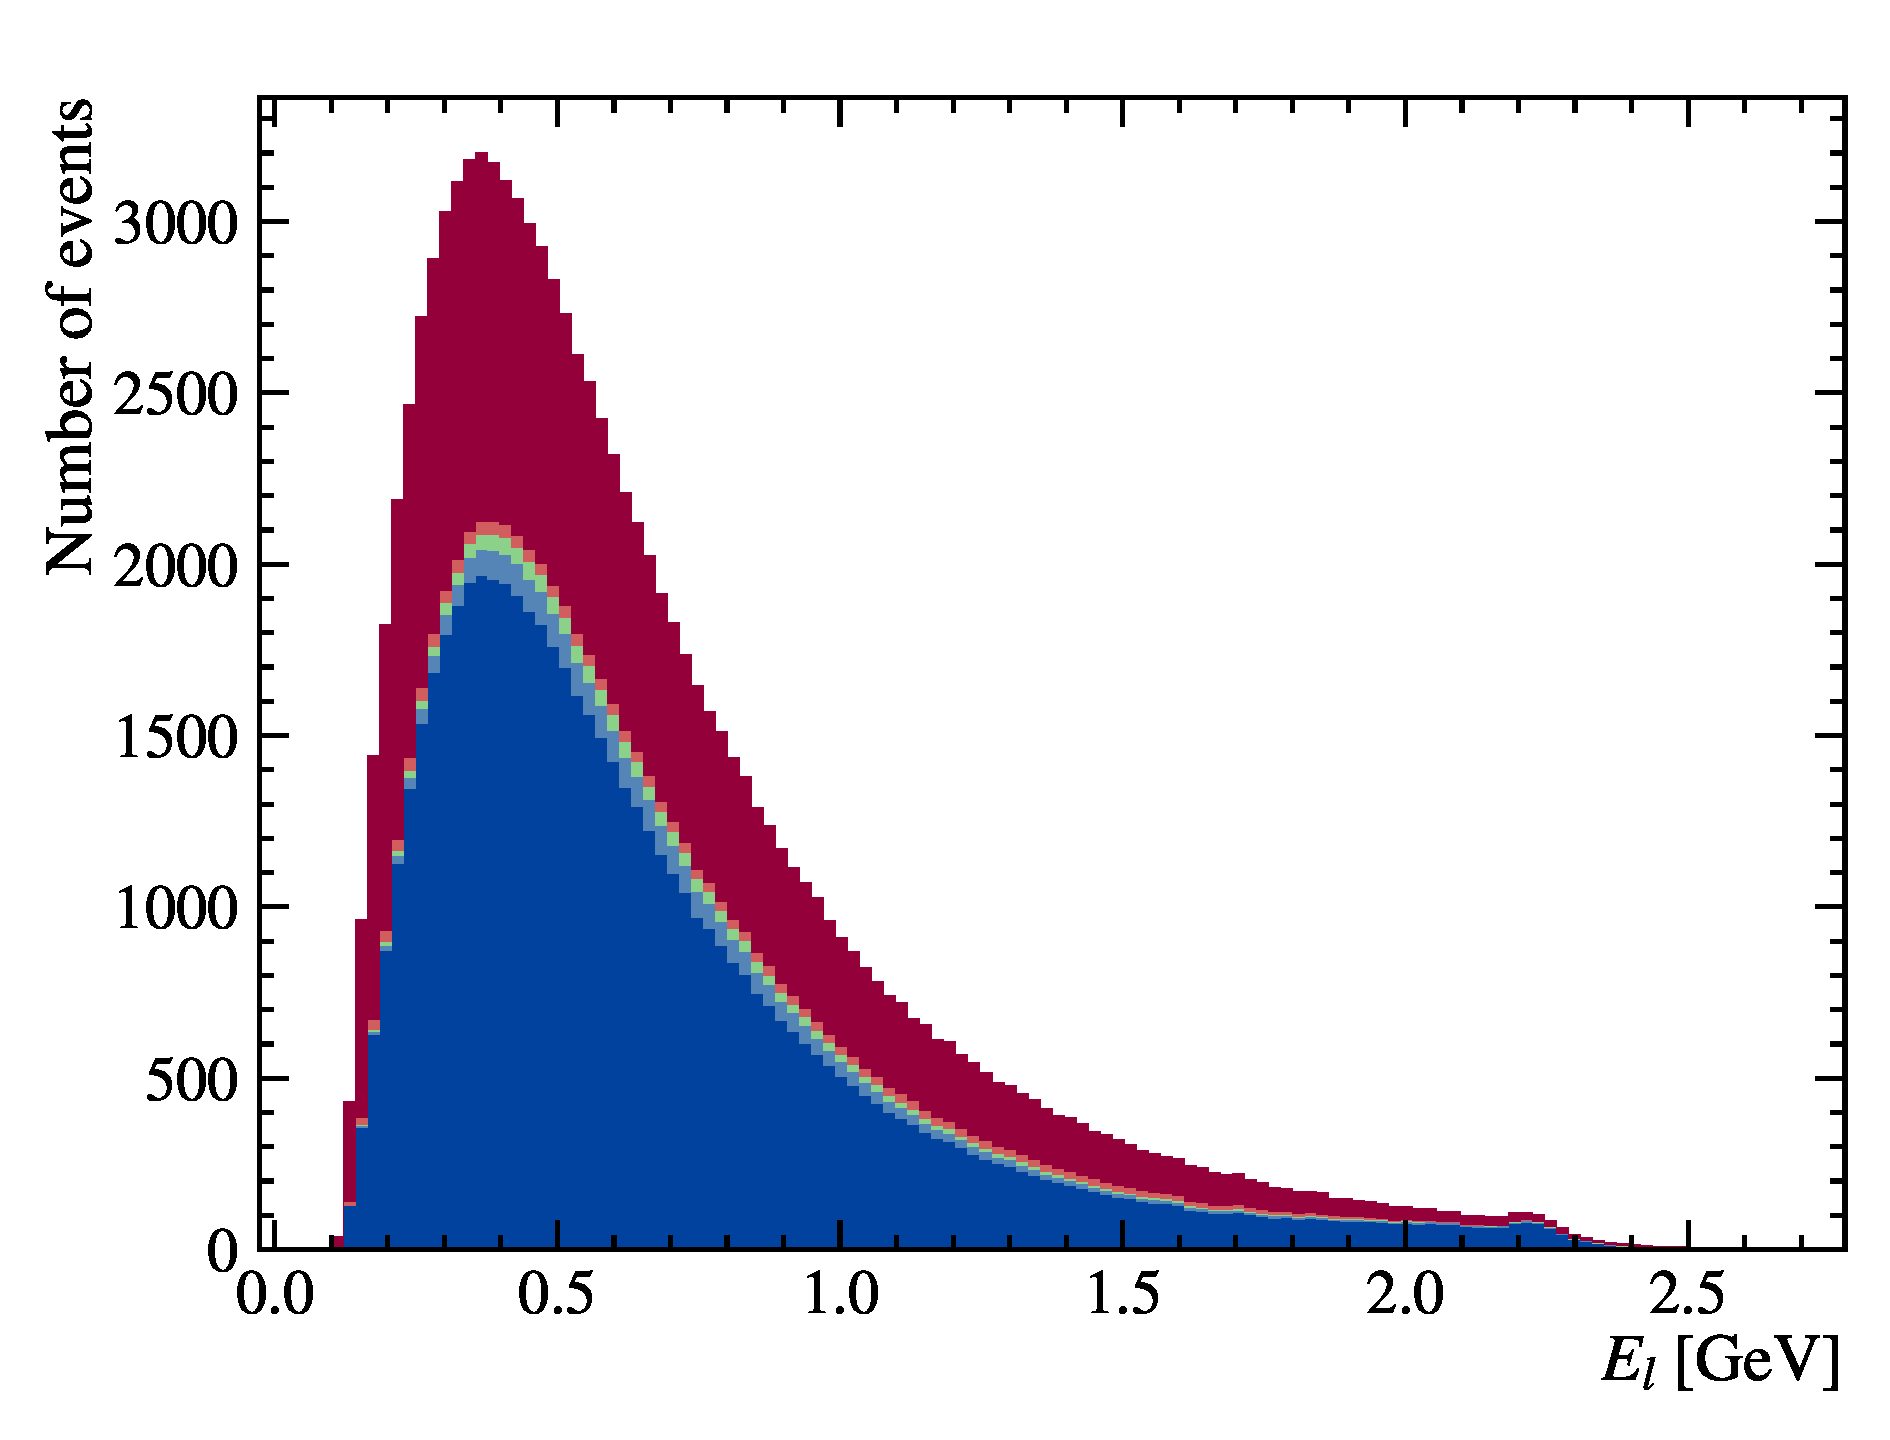
\includegraphics[width=\textwidth]{figs-fit-fit-templates/data-driven-plots/misid/D0_el}
    \end{subfigure}
    \hfill
    \begin{subfigure}[b]{0.32\textwidth}
        \centering
        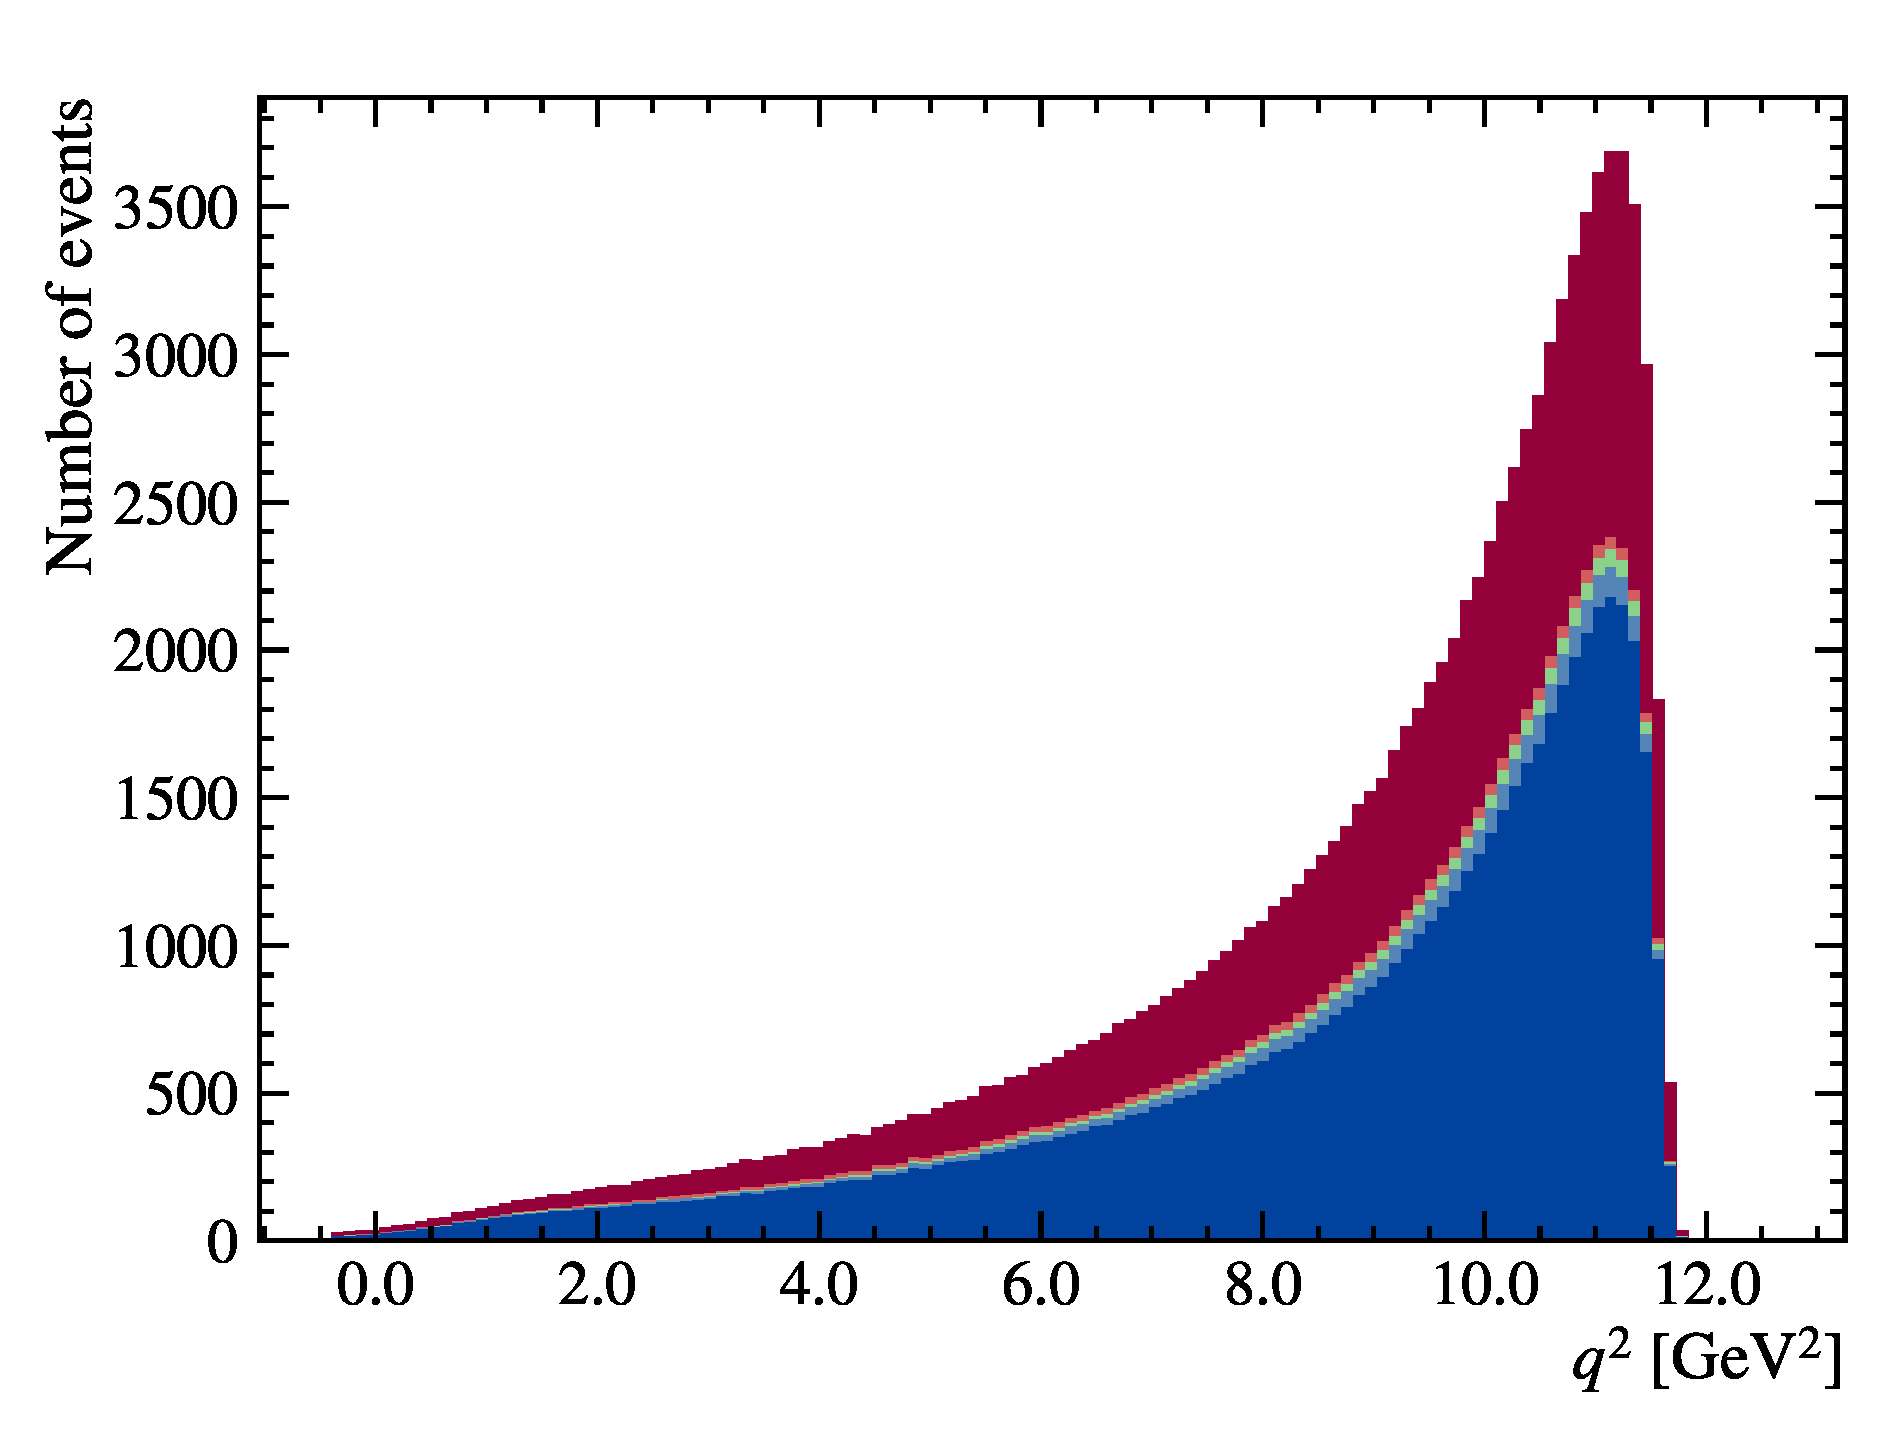
\includegraphics[width=\textwidth]{figs-fit-fit-templates/data-driven-plots/misid/D0_q2.pdf}
    \end{subfigure}
    \caption[Weighted yields of fake \muon sample.]{
        The weighted yields of each species of fake \muon sample projected in
        fit variables.
        The dominate contributions to the ``real'' muon samples are from
        \pion-like and ghost-like tracks.
        The binning are finer compared to \cref{fig:misid-vs-sig}. Actual
        yields are displayed without any rescaling.
    }
    \label{fig:unfolding-fit-vars}
\end{figure}

\begin{table}[htb]
    \centering
    \caption{Selections for each tagged species in fake \muon sample.}
    \label{tab:selection-for-tagged-species}
    \begin{tabular}{crl}
        \toprule
        {\bf Tagged species} & {\bf Variable}            & {\bf Selection} \\
        \midrule
        $\pi$                & \ProbNN{\pion}            & $> 0.1$   \\
                             & \PID{\kaon}               & $< 0.0$   \\
                             & \PID{$p$}                 & $< 0.0$   \\
                             & \PID{$e$}                 & $< 2.0$   \\
                             & \ProbNN{ghost}            & $< 0.25$  \\
        \midrule
        $K$                  & \ProbNN{\kaon}            & $> 0.1$   \\
                             & \PID{\kaon}               & $> 0.0$   \\
                             & \PID{$p$} $-$ \PID{\kaon} & $< 0.0$   \\
                             & \PID{$e$} $-$ \PID{\kaon} & $< -2.0$  \\
                             & \ProbNN{ghost}            & $< 0.25$  \\
        \midrule
        $p$                  & \ProbNN{$p$}              & $> 0.1$   \\
                             & \PID{$p$}                 & $> 0.0$   \\
                             & \PID{$p$} $-$ \PID{\kaon} & $> 2.0$   \\
                             & \PID{$e$} $-$ \PID{$p$}   & $< -2.0$  \\
                             & \ProbNN{ghost}            & $< 0.25$  \\
        \midrule
        $e$                  & \PID{$e$}                 & $> 2.0$   \\
                             & \PID{$e$} $-$ \PID{\kaon} & $> -2.0$  \\
                             & \PID{$e$} $-$ \PID{$p$}   & $> -2.0$  \\
                             & \ProbNN{ghost}            & $< 0.25$  \\
        \midrule
        ghost                & Not in any species above  & \\
        \bottomrule
    \end{tabular}
\end{table}


\subsection{Combinatorial backgrounds}
\label{ref:fit:tmpl:comb}

The selection procedures for all combinatorial backgrounds are listed
in \cref{ref:sel:data:ws}.
The generation procedure for these templates is documented below.
A comparison between combinatorial backgrounds and signal templates is
shown in \cref{fig:comb-vs-sig}.

% TODO: Implement comb. bkg. tmpl. comparison
\begin{figure}[htb]
    \centering
    \begin{subfigure}[t]{0.9\textwidth}
        \centering
        \caption{
            \BComb and \DstComb vs. $\Bm \rightarrow \Dz\taum\neutb$ in \Dz channel.
        }
    \end{subfigure}

    \begin{subfigure}[t]{0.9\textwidth}
        \centering
        \caption{
            \BComb vs. $\Bzb \rightarrow \Dstarp\taum\neutb$ in \Dstar channel.
        }
    \end{subfigure}

    \caption{
        Comparison between combinatorial backgrounds and signal template.
    }
    \label{fig:comb-vs-sig}
\end{figure}

\subsubsection{$D^*$ combinatorial}
\label{dst-comb}

The $D^*$ combinatorial background (\DstComb) arises from a reconstructed $D^0$
combining with an random slow $\pi$, forming a fake $D^*$ vertex and
passing all selection requirements.

The shape of \DstComb can be determined from wrong-sign $\pi$ (WS $\pi$) control
sample which contains mostly $D^0 \pi^-$ pairs.
Still, the yields of \DstComb between nominal right-sign (RS) sample and
WS $\pi$ are not the same,
likely due to differences in selection efficiencies.
Thus a fit on the RS sample is performed to obtain
the yield of \DstComb, then the WS $\pi$ is rescaled to match the fitted yield.
The fit procedure is the following:

\begin{enumerate}
    \item Remove misID contribution from RS sample.
    \item Remove misID contribution from WS $\pi$ sample\footnote{
            A WS $\pi$ control sample from misID sample is reconstructed to
            obtain the misID contribution for data WS $\pi$.
        }.
    \item Fit the mass window $m_{D^*} - m_{D^0}$ (including events normally
        outside the window) on RS sample with a
        double-Gaussian signal and an exponential background.
        The background yield under the mass window where a $D^*$ is nominally
        accepted is taken as the yield of \DstComb.

        The fit to ISO skim is shown in \cref{fig:dst-comb-fit}.
        The effect of scaling for the ISO skim is shown in
        \cref{fig:dst-comb-scale}.
        For fit to 1OS, 2OS, and DD skims, refer to \cref{appx:suppl:dst-comb}.
\end{enumerate}

\techlink{appx:tech:fit-to-comb-bkg}

% Generated in /rdx-run2-analysis/fit with the command:
%   make fit-DstComb
\begin{figure}[htb]
    \centering
    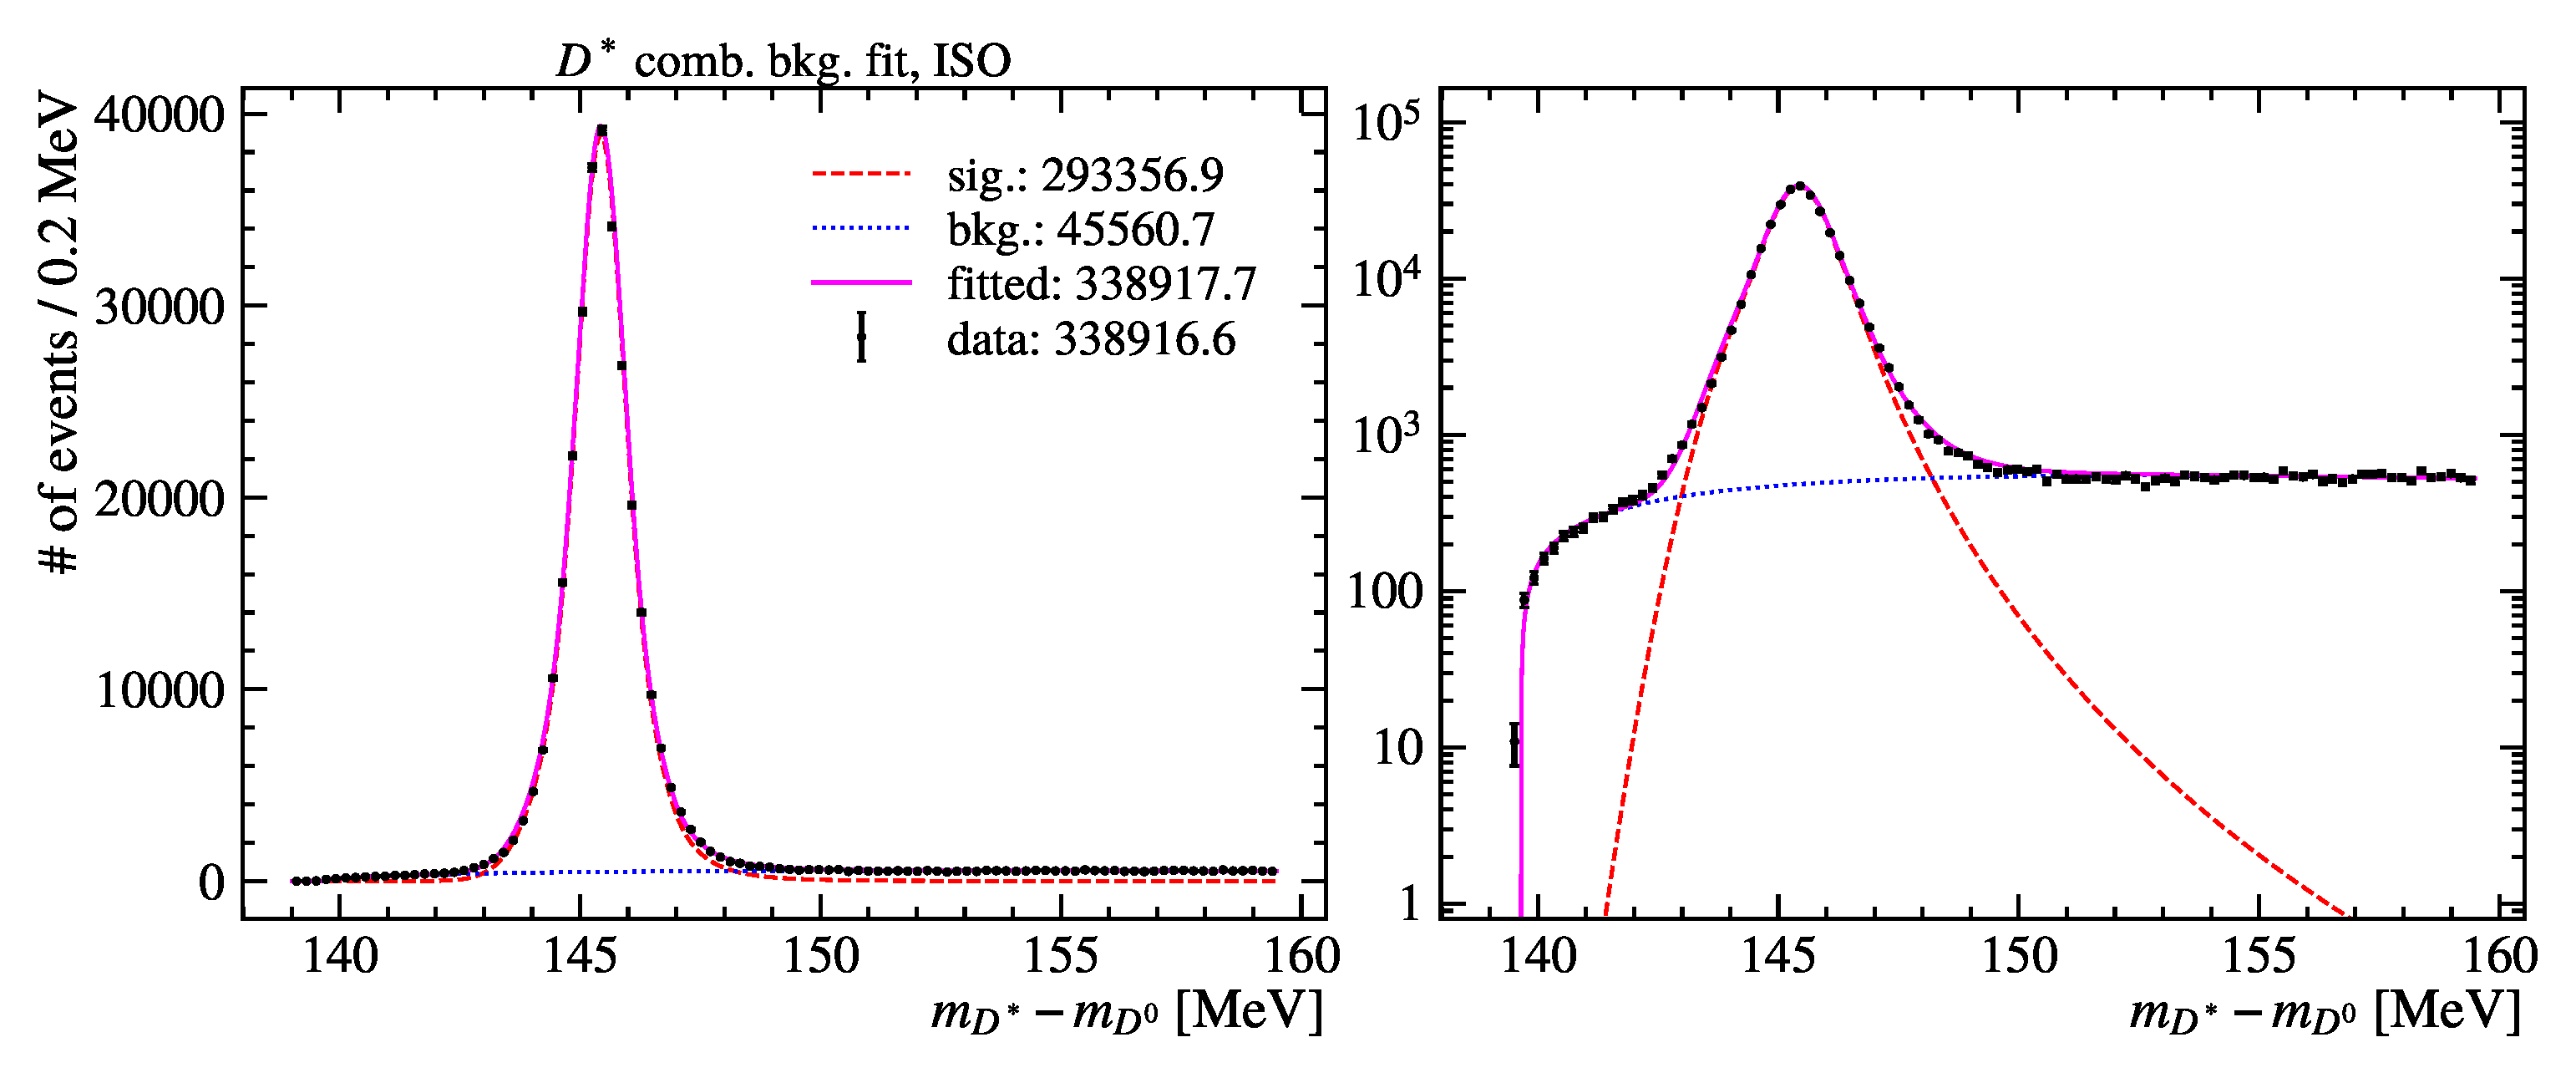
\includegraphics[width=\textwidth]{figs-fit-fit-templates/data-driven-plots/dst_comb/fit_dst_comb_iso_comb.pdf}
    \caption{
        \DstComb\ auxiliary fit to the ISO skim.
        Right plot shows the same fit as in the left, but with a logarithmic $y$
        axis.
    }
    \label{fig:dst-comb-fit}
\end{figure}

\begin{figure}[htb]
    \centering
    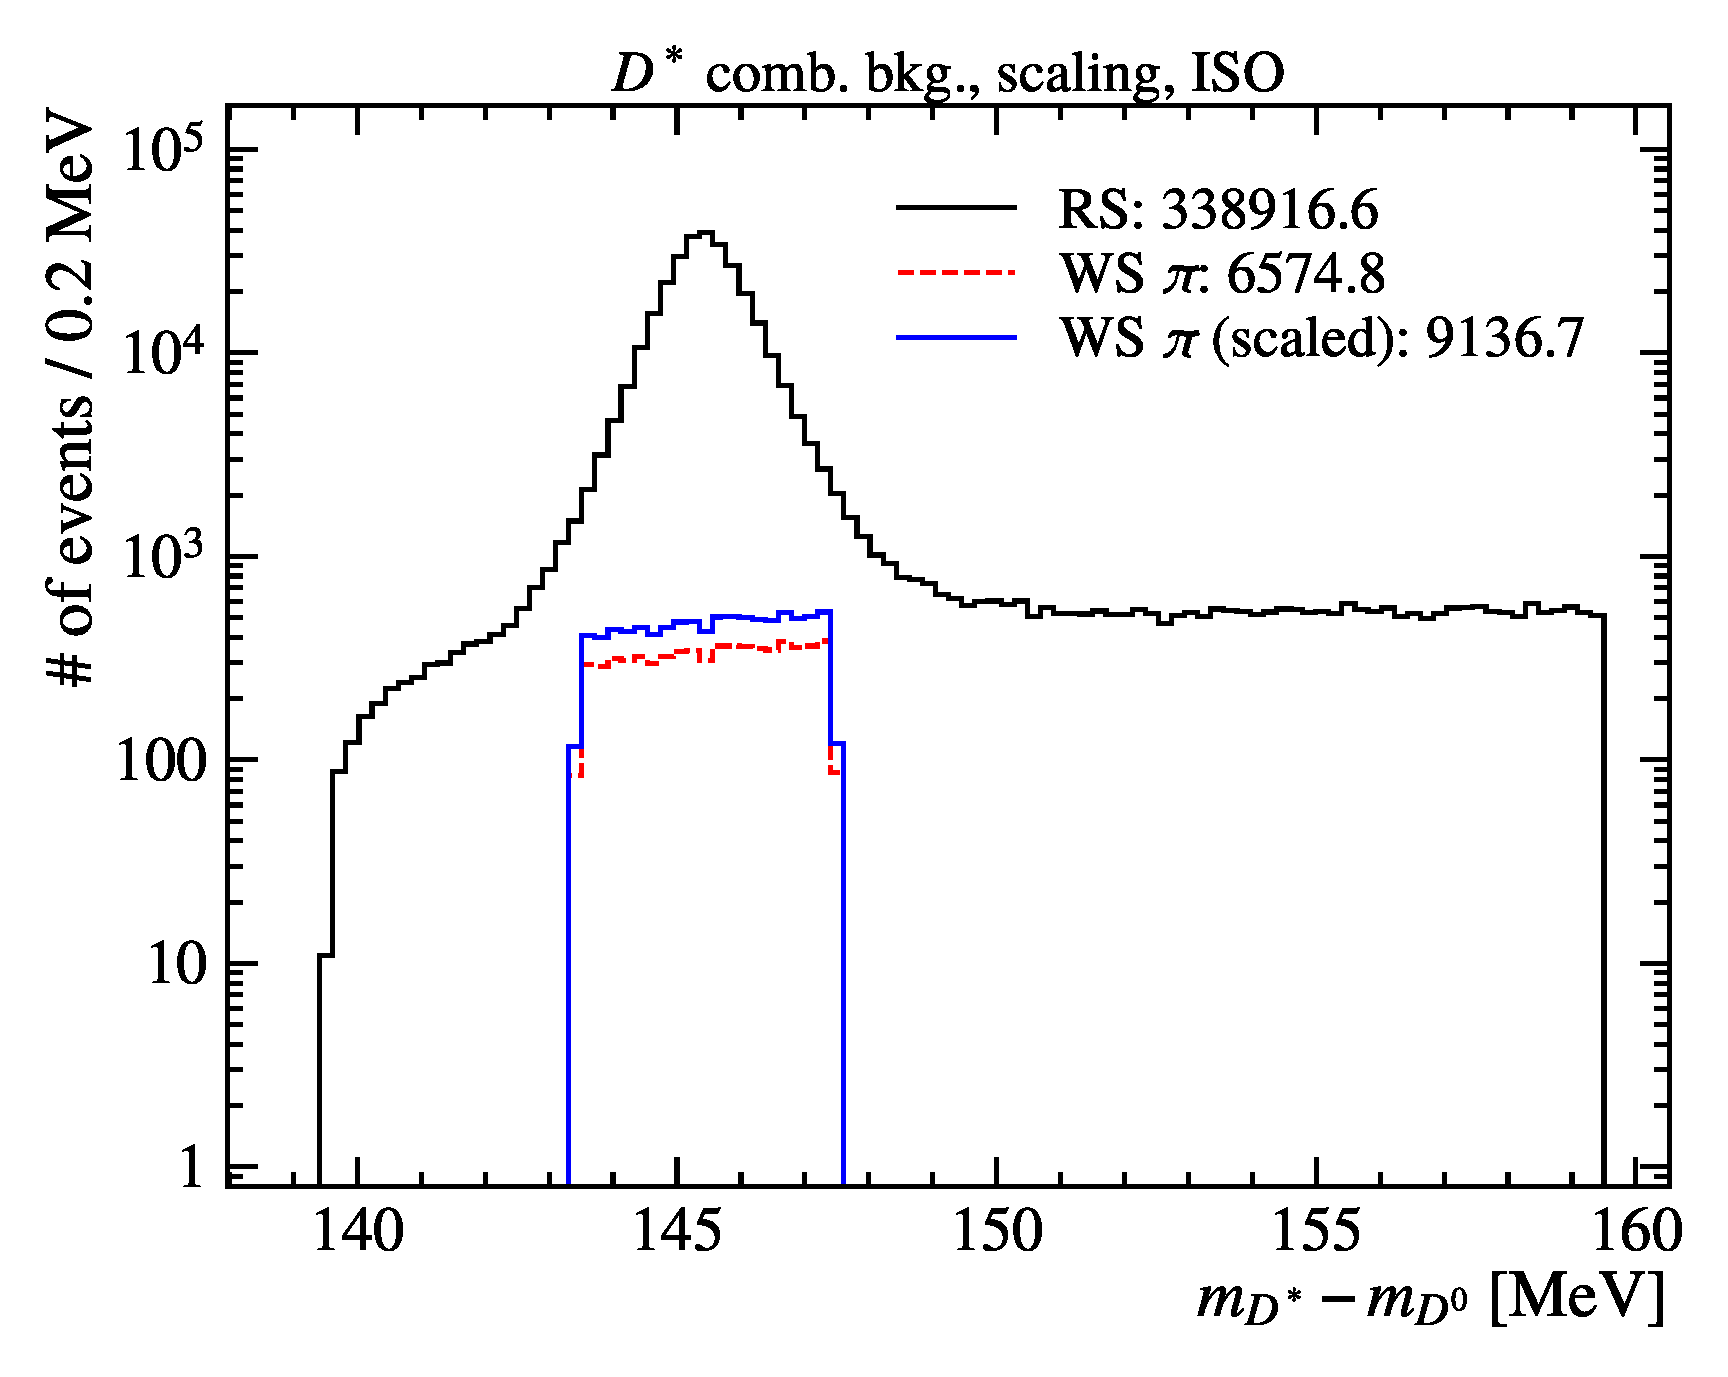
\includegraphics[width=0.55\textwidth]{figs-fit-fit-templates/data-driven-plots/dst_comb/fit_dst_comb_scaled_comp_iso_log.pdf}
    \caption{
        Effect of scaling for the ISO skim on the \DstComb\ template.
    }
    \label{fig:dst-comb-scale}
\end{figure}

\subsubsection{$B$ combinatorial in $D^*$ channel}
\label{b-comb-dst}

The $B$ combinatorial (\BComb) in $D^*$ fit channel comes from randomly
combined $D^* \mu$ pairs.
Again, the shape of the \BComb\ is determined by wrong-sign $\mu$ (WS $\mu$)
control sample containing $D^{*+} \mu^+$ pairs.

Further, it is assumed that the \BComb\ from WS $\mu$ and \BComb\ from RS
differs by a factor linear in $m_B$.
This is justified by assuming \BComb\ are slow-varying exponential decays in
terms of $m_B$ for both RS and WS $\mu$, thus the ratio between the two is also
an exponential.
Since they are slow-varying, Taylor expansion to the first order (i.e. of the
form $a + b m_B$) agrees well with the ratio in a sufficiently large region.

Unlike $m_\Dstar$ in \DstComb,
$m_B$ does not have a clear lower side-band.
This is because \B is only \emph{partially} reconstructed
due to missing neutrino(s).
Therefore, only the upper-sideband, defined as $m_B > 5400$ MeV,
which contains purely combinatorial and misID, can be used to
study \BComb.

A fit is performed in $B$ mass upper-sideband  to obtain
the linear scaling factor $a + b m_B$.
In the upper-sideband, it is assumed that both WS $\mu$ and RS samples contain
are pure, that is, containing only combinatorial backgrounds and misID.
The linear scaling factor is assumed to be the same for all skims\footnote{
    This is mainly because there is not enough number of events in the
    upper-sideband to perform fits skim-by-skim.
}.
The fit is performed in the following manner:

\begin{enumerate}
    \item Remove misID contribution from RS sample.
    \item Remove misID contribution from WS $\mu$ sample.
    \item Perform a fit on RS sample in the upper-sideband region to determine
        contribution from \DstComb, with procedure identical to that in
        \cref{dst-comb}.
        Then remove the fitted \DstComb.
    \item Fit and remove \DstComb\ from WS $\mu$ sample.
    \item Compute the ratio between RS and WS $\mu$, perform a fit to obtain
        the linear scaling factor.
        The fit, as well as
        The raw RS and WS $\mu$ templates, as well as scaled WS $\mu$
        template, is shown in \cref{fig:b-comb-dst}.
\end{enumerate}

% FIXME: Replace quad. fit w/ an exp. fit
% Generated in /rdx-run2-analysis/fit with the command:
%   make fit-BCombDst
\begin{figure}[htb]
    \centering
    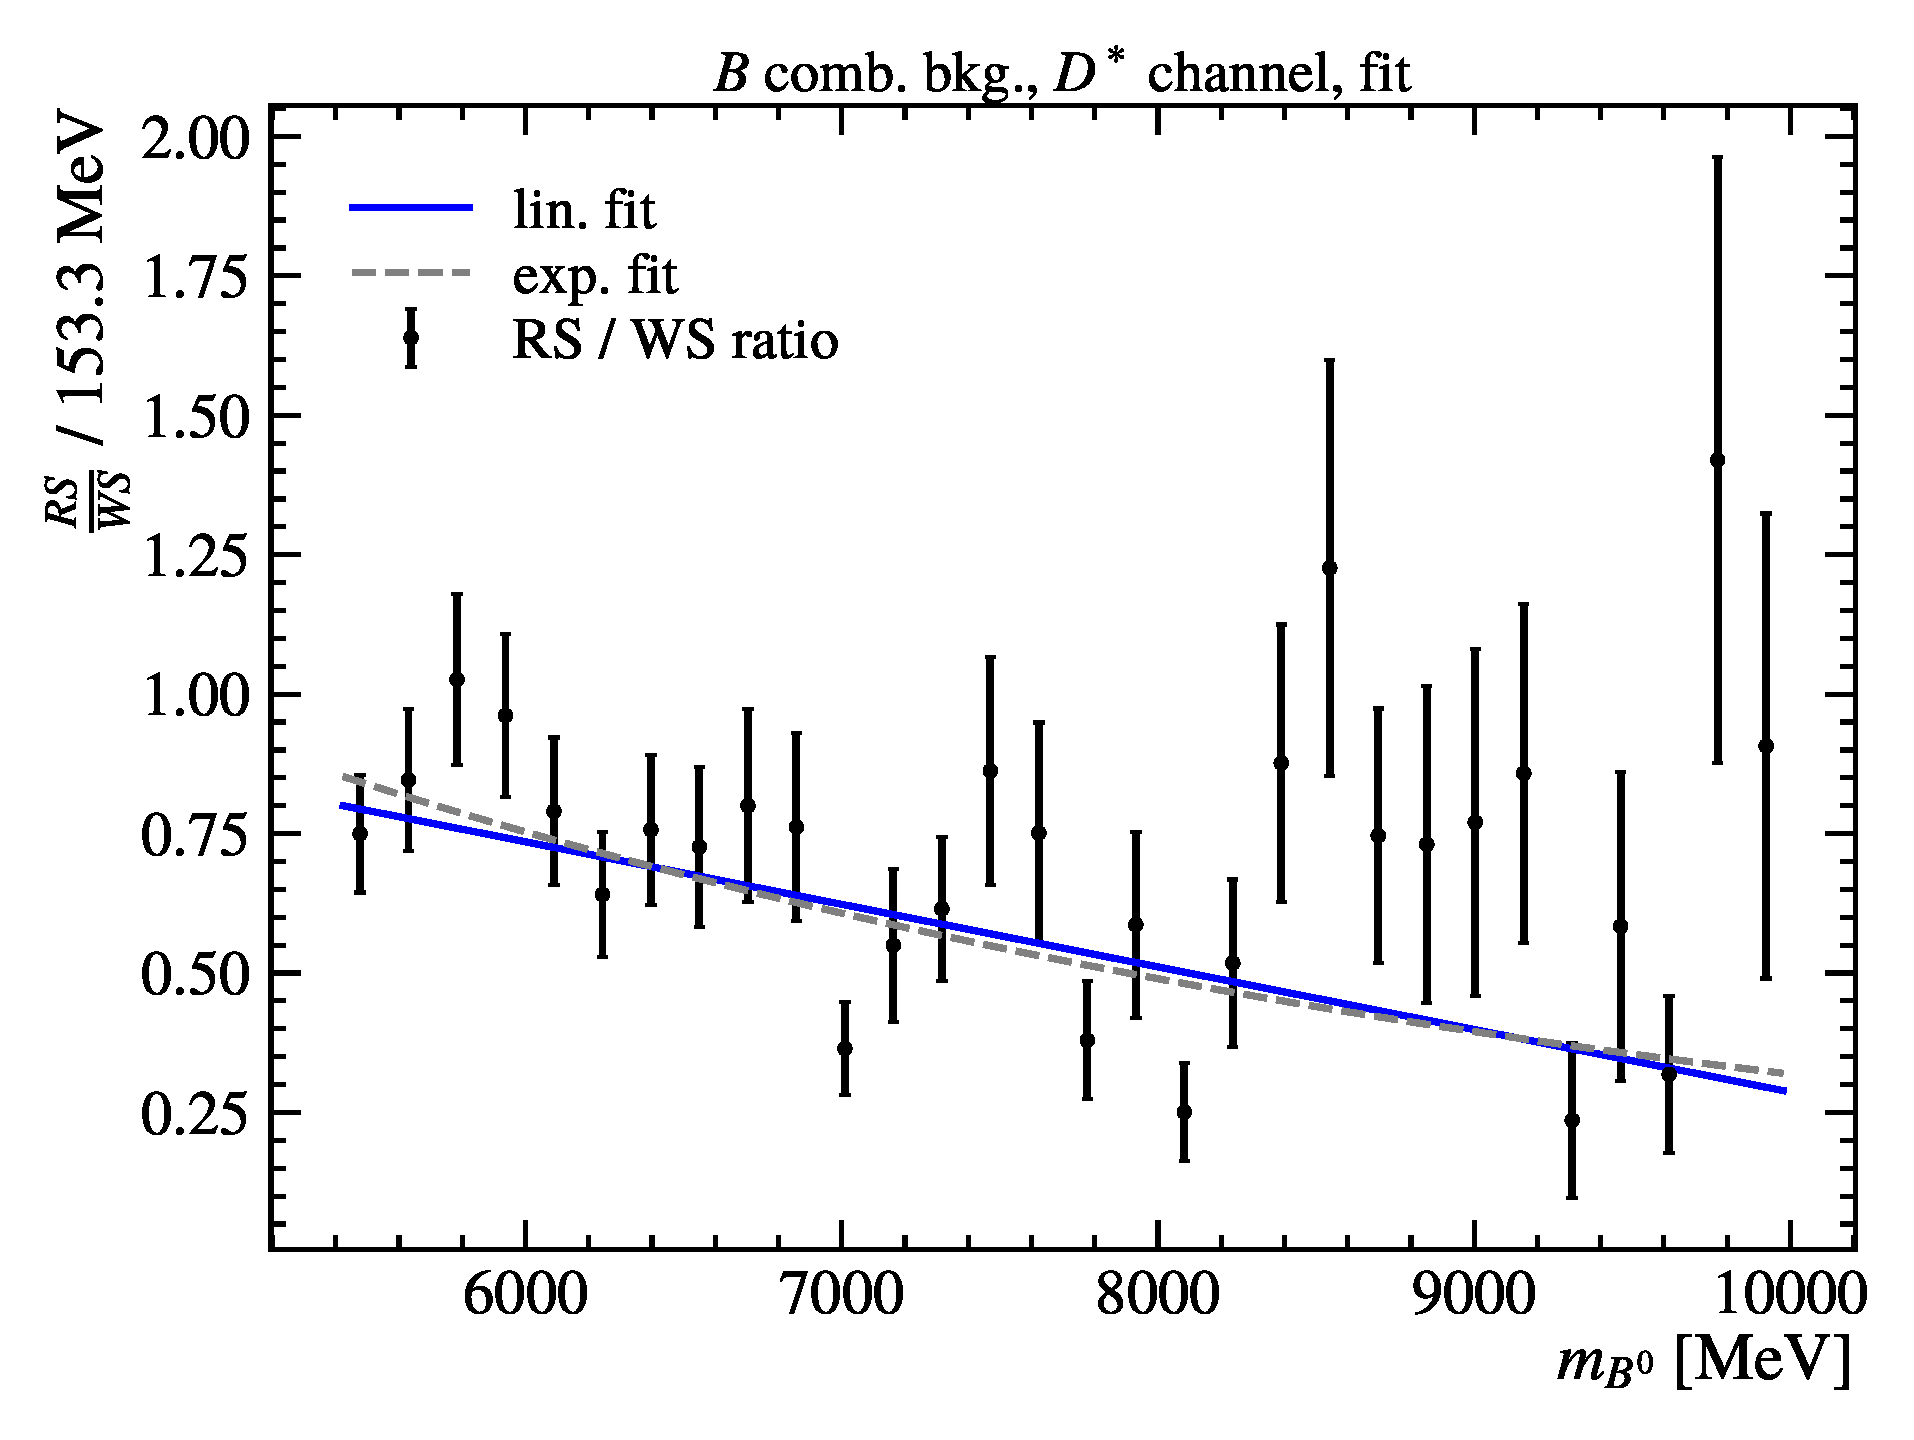
\includegraphics[width=0.48\textwidth]{figs-fit-fit-templates/data-driven-plots/b_comb/fit_b_comb_dst_fit.pdf}
    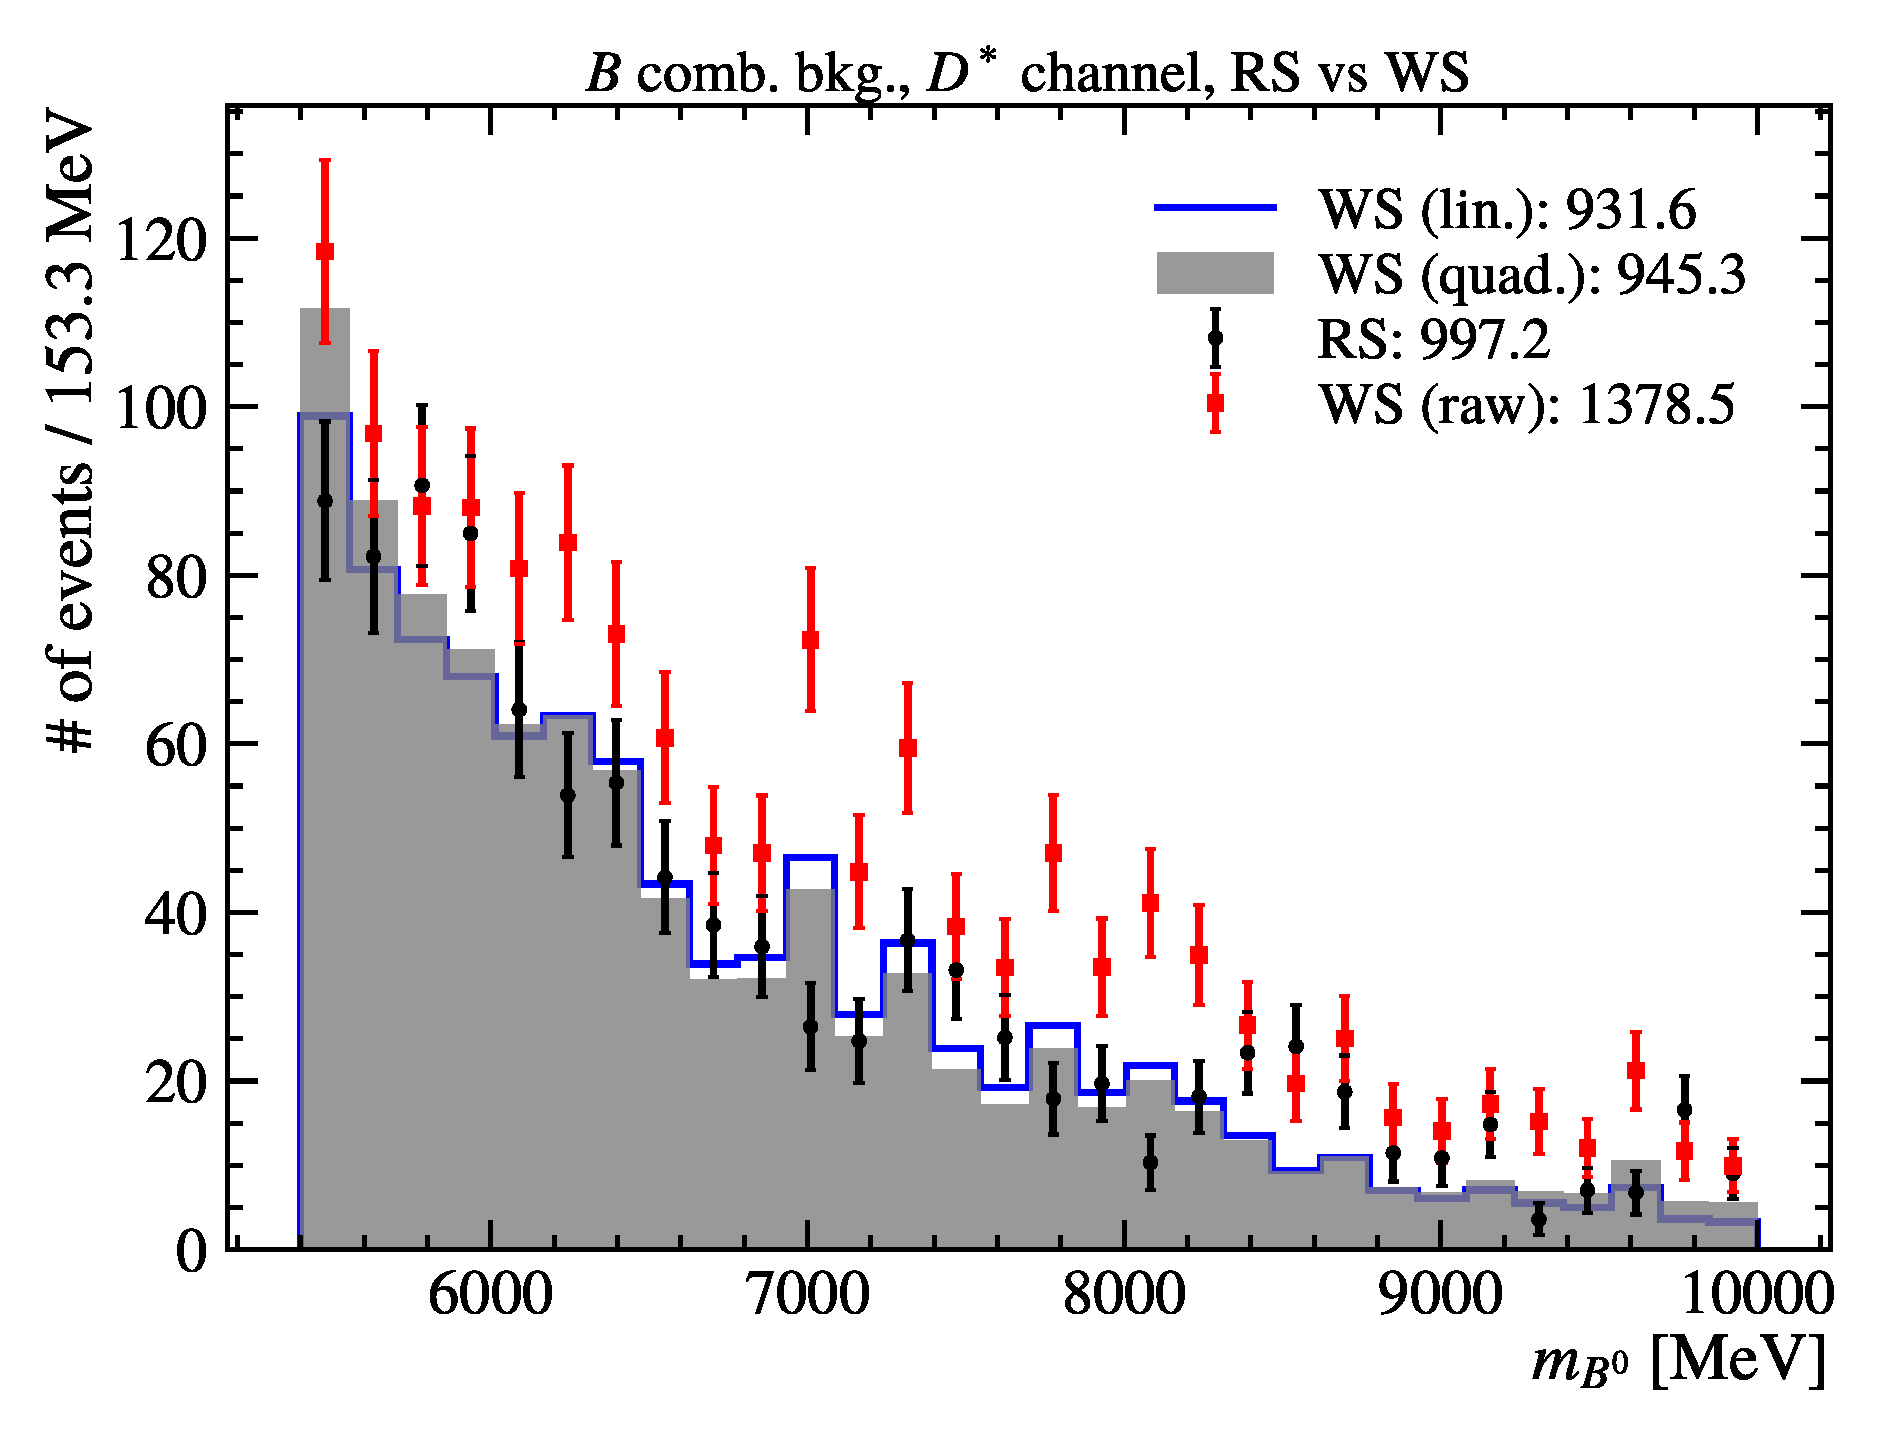
\includegraphics[width=0.48\textwidth]{figs-fit-fit-templates/data-driven-plots/b_comb/fit_b_comb_dst_scaled.pdf}

    \caption[\BComb\ fit result for $D^*$ channel]{
        \BComb\ fit result for $D^*$ channel.

        Left: \BComb\ auxiliary fit in the $m_B$ upper-sideband region for all skims.
        A quadratic fit is also performed for possible systematic studies.

        Right: The scaling effect on the WS $\mu$ \BComb\ template.
    }
    \label{fig:b-comb-dst}
\end{figure}

\subsubsection{$B$ combinatorial in $D^0$ channel}
\label{b-comb-d0}

The procedure is similar to that in \cref{b-comb-dst}, but without \DstComb\
removal. The fit is shown in \cref{fig:b-comb-d0}.

% FIXME: Replace quad. fit w/ an exp. fit
% Generated in /rdx-run2-analysis/fit with the command:
%   make fit-BCombD0
\begin{figure}[htb]
    \centering
    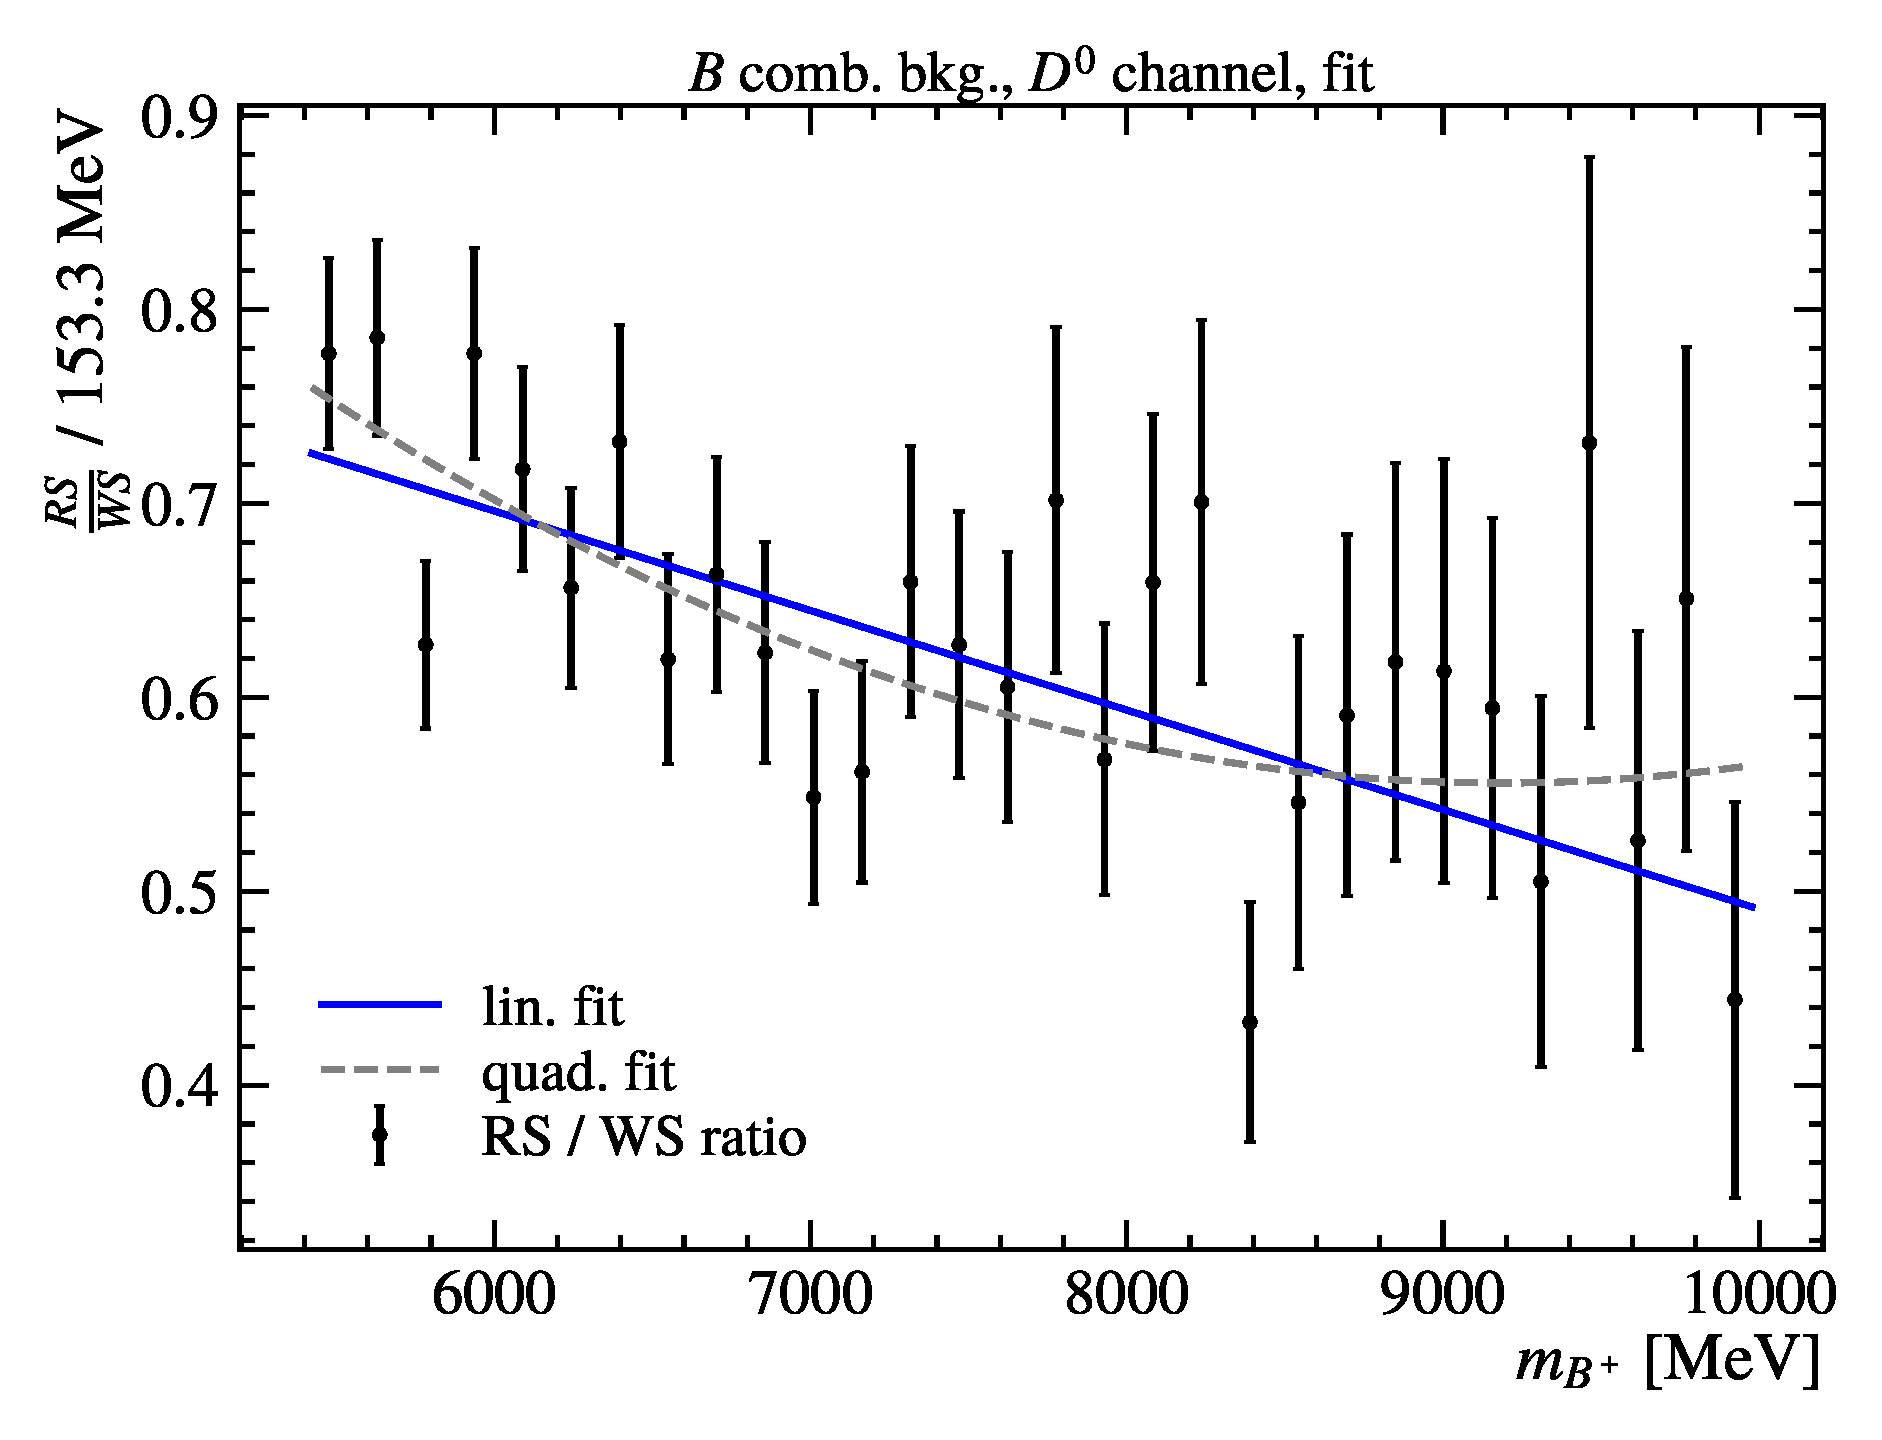
\includegraphics[width=0.48\textwidth]{figs-fit-fit-templates/data-driven-plots/b_comb/fit_b_comb_d0_fit.pdf}
    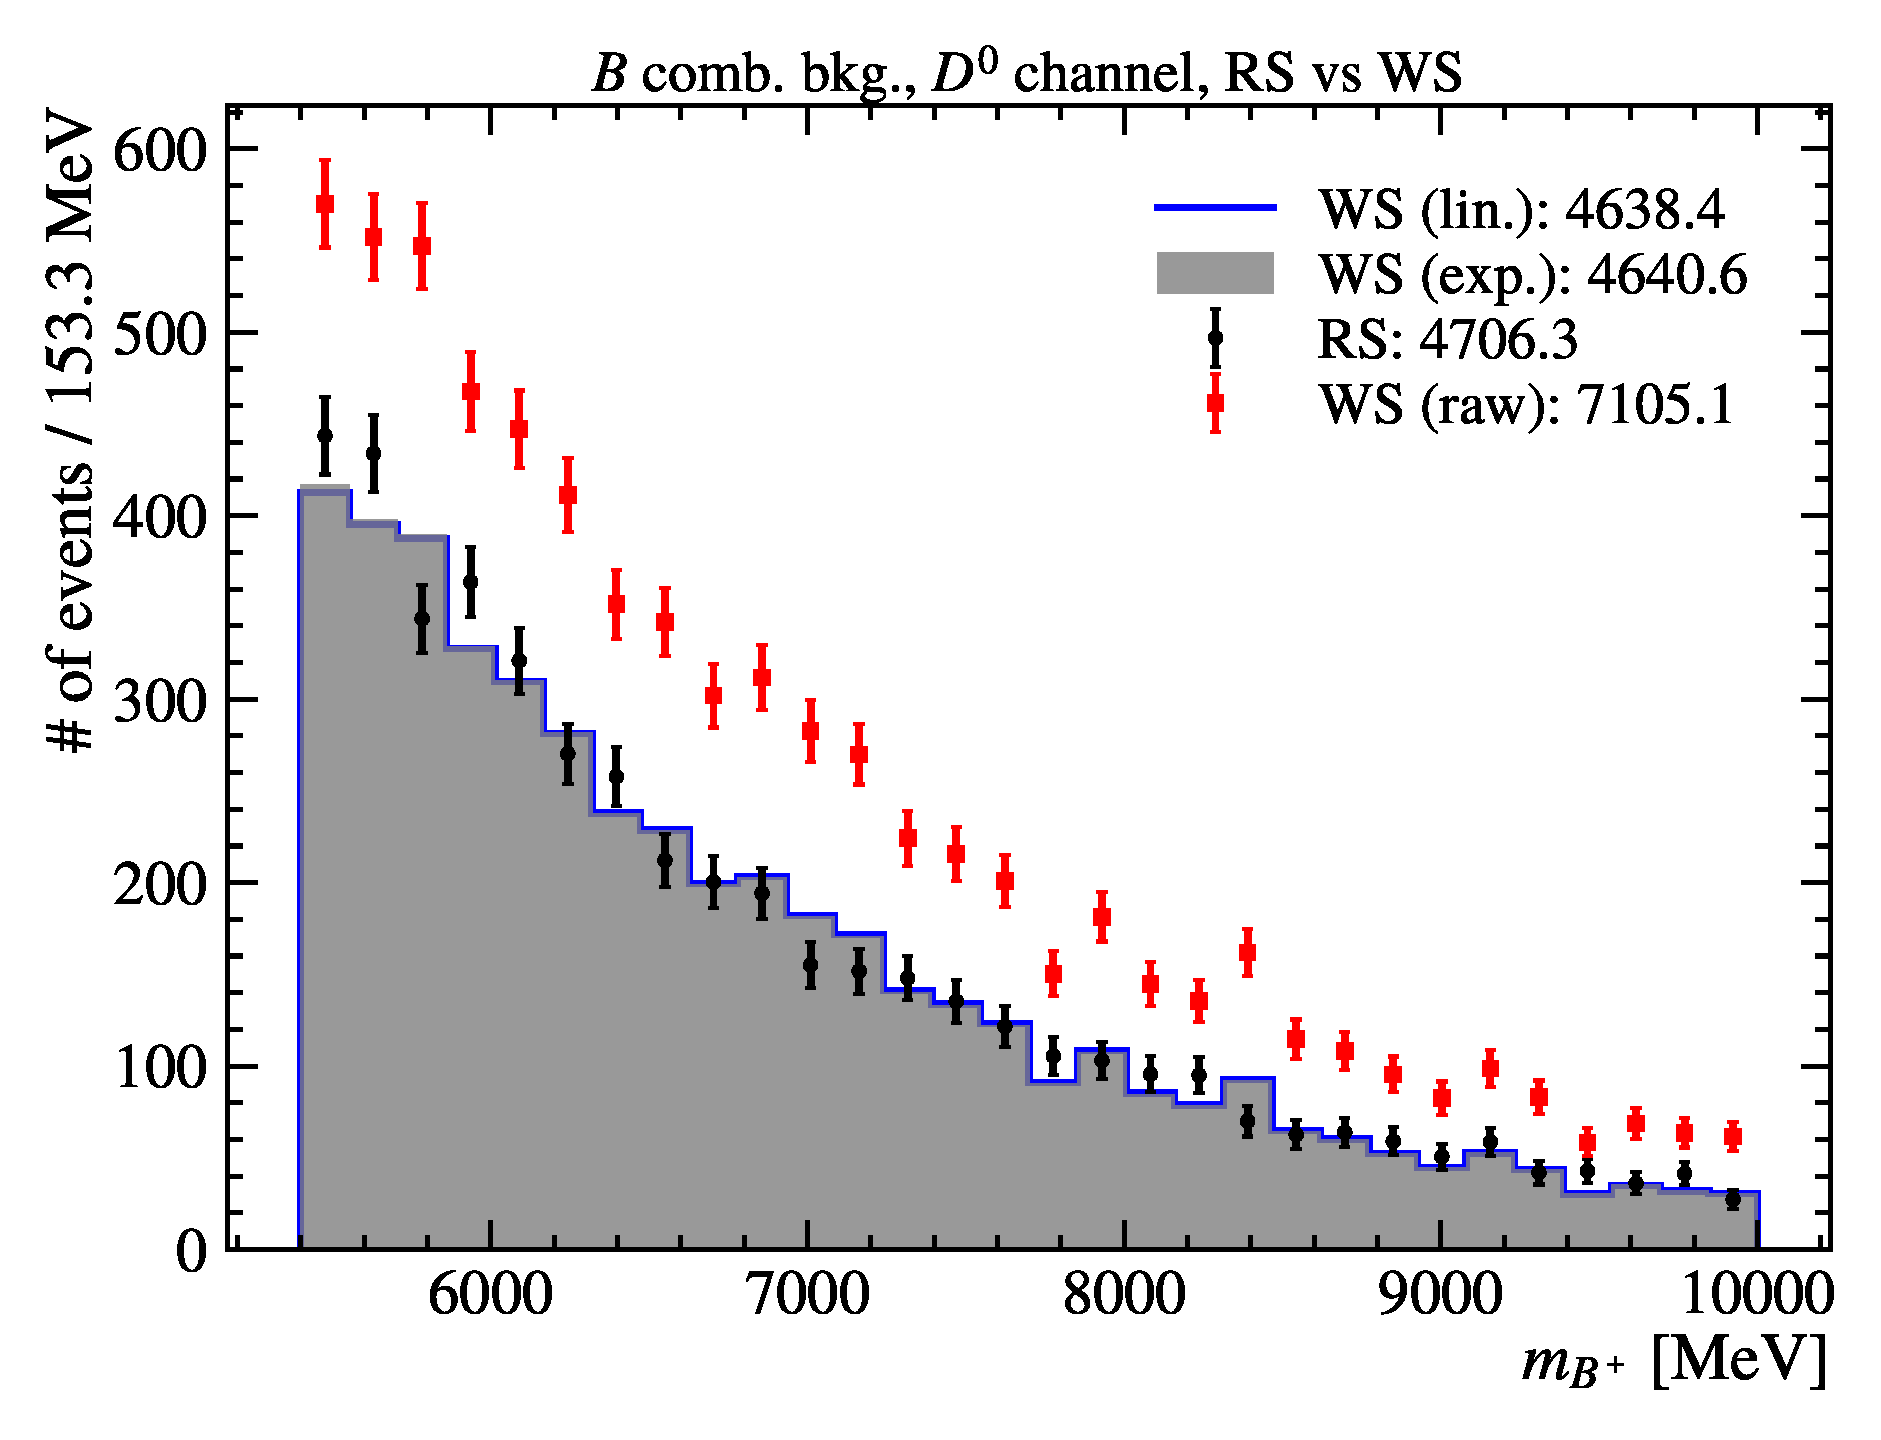
\includegraphics[width=0.48\textwidth]{figs-fit-fit-templates/data-driven-plots/b_comb/fit_b_comb_d0_scaled.pdf}

    \caption{
        \BComb\ fit result for $D^*$ channel.
        Left: \BComb\ auxiliary fit.
        Right: The scaling effect on the WS $\mu$ \BComb\ template.
    }
    \label{fig:b-comb-d0}
\end{figure}


\subsection{Signal and normalization}
\label{tmpl:sig-norm}

\paragraph{$B \rightarrow D^{0,*+}\mun\neumb$}
These are normalization templates.
The yields of these two modes, denoted as $N_{D\mu}$ and $N_{\Dstar\mu}$,
are set to be the free-floating overall normalization of the respective
fit channels.
As a side, the \Dz\muon template has notably softer \qSq spectrum compared to
that of \Dstar\muon, due to reduced helicity states available in the
$B \rightarrow D \ell \neulb$ transitions
(discussed in \cref{ref:theory:ff-d0-dst}),
as shown in \cref{fig:d0-norm-vs-dst-norm}.
The \Dstarp templates (both muonic and tauonic) contribute to both fit channels
due to feed down.

\begin{figure}[htb]
    \caption{
        Comparison between $\Bm \rightarrow \Dz\mun\neumb$ and
        $\Bzb \rightarrow \Dstarp\mun\neumb$ templates.
    }
    \label{fig:d0-norm-vs-dst-norm}
\end{figure}

\paragraph{$B \rightarrow D^{0,*+}\taum\neutb$}
The signal templates, with \RD and \RDstp controlling the fraction
of yields compared to respective normalization yields.
The signal distributions are characterized by high \mmSq and softer
\el (due to \muon coming from a \tauon decay),
as shown in \cref{fig:d0-sig-vs-d0-norm,fig:dst-sig-vs-dst-norm}.
Also, the \Dz\tauon has a softer \qSq distribution, due to the same reason
mentioned in the normalization comparison, which is displayed in
\cref{fig:d0-sig-vs-dst-sig,fig:d0-sig-vs-dst0-sig}.

\begin{figure}[htb]
    \begin{subfigure}{\textwidth}
        \caption{
            $\Bm \rightarrow \Dz\mun\neumb$ vs.
            $\Bm \rightarrow \Dz\taum\neutb$.
        }
        \label{fig:d0-sig-vs-d0-norm}
    \end{subfigure}

    \begin{subfigure}{\textwidth}
        \caption{
            $\Bzb \rightarrow \Dstarp\mun\neumb$ vs.
            $\Bzb \rightarrow \Dstarp\taum\neutb$.
        }
        \label{fig:dst-sig-vs-dst-norm}
    \end{subfigure}

    \begin{subfigure}{\textwidth}
        \caption{
            $\Bm \rightarrow \Dstarz\mun\neumb$ vs.
            $\Bm \rightarrow \Dstarz\taum\neutb$.
        }
        \label{fig:dst0-sig-vs-dst0-norm}
    \end{subfigure}
    \caption{Comparison between signal and normalization templates.}
\end{figure}

\begin{figure}[htb]
    \begin{subfigure}{\textwidth}
        \caption{
            $\Bm \rightarrow \Dz\taum\neutb$ vs.
            $\Bzb \rightarrow \Dstarp\taum\neutb$.
        }
        \label{fig:d0-sig-vs-dst-sig}
    \end{subfigure}

    \begin{subfigure}{\textwidth}
        \caption{
            $\Bm \rightarrow \Dz\taum\neutb$ vs.
            $\Bm \rightarrow \Dstarz\taum\neutb$.
        }
        \label{fig:d0-sig-vs-dst0-sig}
    \end{subfigure}

    \caption{Comparison between signal templates.}
\end{figure}

\paragraph{$\Bm \rightarrow D^{*0}\ellm\neulb$}
The \Dstarz ($\rightarrow \Dz \pi$ or $\rightarrow \Dz \gamma$)
in these modes are not reconstructed,
so these templates contribute to the \Dz channel only.
The muonic mode contains an additional branching fraction ratio on top of
$N_{D\mu}$ in its normalization, and is the largest class of contribution
in \Dz data.
For tauonic mode, the \RDstz is set to be equal to \RDstp in the nominal fit.


\subsection{Feed down through $B \rightarrow D^{**}\ellm\neulb$ modes}
\label{tmpl:dstst}

% FIXME: D** descr is pretty bad!
The feed downs from 4 $1P$ $D^{**}$ states
($D_1(2420), D_2^*(2460), D_0^*(2430), D'_1(2430)$, including both isospin
pairs) are included in the fit,
with $10+10$ ($\mu+\tau$) templates in \Dz channel
and $6+6$ in \Dstar.
These $D^{**}$ decay into a \Dz either directly or in a
cascade via a \Dstar or a lighter $D^{**}$,
possibly producing two \emph{charged} \pion
(hence the \Dz\pion\pion templates).

\paragraph{Muonic}
The $D^{**}$ decays often contain unreconstructed \piz or $\gamma$ which leads
to a broad \mmSq distribution peaking at smaller values $\approx m^2_\pion$,
as shown in \cref{fig:dstst-mu-vs-d0-sig}.
The \el spectrum is comparable, but typically softer, than that in normalization,
due to $D^{**}$ states having higher masses compared to \Dz and \Dstar.
These decays are suppressed at zero recoil, as discussed in
\cref{ref:theory:ff-dstst},
but translates weakly in the reconstructed \qSq spectrum, due to rest frame
approximation (\cref{appx:rfa}) and definition of \qSq being
$(p_B - p_D)^2$, instead of $(p_B - p_{D^{**}})^2$.

Currently, the constraints for these modes are
taken from the run 1 analysis (\cite{LHCb-ANA-2020-056}), which uses PDG data.
For each sample (i.e. ISO, 1OS, 2OS, DD),
%It is worth noting that a factor
%$n^{0,*}_{D^{**}} \equiv 10^{-3} / \mathcal{B}(B \rightarrow D^{0,*}\mun\neumb)$
%is include such that floating parameters may be read as a branching fractions
%times an efficiency directly.

\begin{figure}[htb]
    %\begin{subfigure}{\textwidth}
    %    \caption{
    %        $\Bm \rightarrow \Dz\taum\neutb$ vs.
    %        $\Bzb \rightarrow \Dstarp\taum\neutb$.
    %    }
    %    \label{fig:d0-sig-vs-dst-sig}
    %\end{subfigure}

    \caption{Comparison between $D^{**}\mu$ and \Dz\taum signal templates.}
    \label{fig:dstst-mu-vs-d0-sig}
\end{figure}

\paragraph{Tauonic}
As in run 1, the tauonic $D^{**}$ decays are treated as fixed fractions
to their muonic counterparts individually, with each $\mathcal{R}(D^{**})$
fraction given by \cite{Bernlochner_2018} within their ``Approximation C'',
for an weighted average of 0.085.
However, the run 1 \RDst analysis (\cite{LHCb-ANA-2014-052}) used
0.12, instead 0.085,
though the values agree within errors specified in that analysis.
Suffice to say, $R(D^{**})$ ratios are not measured to precision.
Therefore, a Gaussian constraint with a width of 30\% is added,
allowing the yields to float around the nominal values.
The Gaussian constraint is shared among all $1P$ $D^{**}$ species within
each fit channel (e.g. \Dz channel) but is distinct across channels.


\subsection{Feed down through $B \rightarrow D_H^{**}(\rightarrow D^{(*)}\pi\pi)\mun\neumb$ modes}

The heavy $D_H^{**}$ decay into either a \Dz or a \Dstar, with two additional
\pion and one of them possibly uncharged.
The fit variables are distributed similar to that in the lighter
$D^{**}$ states.
A comparison between the $D_H^{**}$ templates and \Dz\taum signal can be
seen at \ref{fig:dstst-heavy-vs-d0-sig}

\begin{figure}[htb]
    %\begin{subfigure}{\textwidth}
    %    \caption{
    %        $\Bm \rightarrow \Dz\taum\neutb$ vs.
    %        $\Bzb \rightarrow \Dstarp\taum\neutb$.
    %    }
    %    \label{fig:d0-sig-vs-dst-sig}
    %\end{subfigure}

    \caption{Comparison between $D_H^{**}\mu$ and \Dz\taum signal templates.}
    \label{fig:dstst-heavy-vs-d0-sig}
\end{figure}


\subsection{Feed down through $\Bsb \rightarrow D_s^{**}\mun\neumb$ modes}

The $D_s^{**}$\footnote{
    More specifically, the $D_{s1}^{'+}$ and $D_{s2}^{*+}$ are included in
    this analysis.
}, daughter of \Bsb, decays into either a $\Kp\Dz$ or $\Kz\Dstarp$.
The former feeds into \Dz channel, whereas the latter feeds into both.
These modes are constrained based on available measurements.
A comparison between the $D_s^{**}$ templates and \Dz\taum signal can be
seen at \cref{fig:d_s-vs-d0-sig}.

\begin{figure}[htb]
    %\begin{subfigure}{\textwidth}
    %    \caption{
    %        $\Bm \rightarrow \Dz\taum\neutb$ vs.
    %        $\Bzb \rightarrow \Dstarp\taum\neutb$.
    %    }
    %    \label{fig:d0-sig-vs-dst-sig}
    %\end{subfigure}

    \caption{Comparison between $D_s^{**}\mu$ and \Dz\taum signal templates.}
    \label{fig:d_s-vs-d0-sig}
\end{figure}


\subsection{Double-charm ($DDX$) backgrounds}
\label{ref:fit:tmpl:ddx}

The double-charm backgrounds include contributions from
$B \rightarrow D^{(*)}(\rightarrow \mun\neumb)\bar{D}^{(*)} X$ decays, where $X$
is either a \kaon, a \Kstar, or a higher \Kstar resonance.
The $DDX$ are poorly understood as these MC are generated with
a phase space model so generated events are distributed evenly in the available
phase space, without taking the resonance structure,
which itself is not precisely known for $n \geq 3$-body decays,
of the Dalitz plane into account.
Additionally, the $D \rightarrow X \ell\neulb$ decay form factors are
parameterized with the quark-model of ISGW2,
which is known to unable describe data sufficiently well\footnote{
    As commented in \cite{LHCb-ANA-2020-056}:
    ``In the current literature it is found that single-pole-dominance provides
    a much better description of the data than quark-model calculations.''
}.
More details regarding the variations will be discussed in
\cref{ref:fit:var:ddx}.
Both muonic and tauonic $DDX$ templates are similar to the signal templates,
as can be seen in \cref{fig:ddx-vs-d0-sig}.
This is due to the fact that a large portion of energy is taken by the
unreconstructed $D$ meson.

\begin{figure}[htb]
    %\begin{subfigure}{\textwidth}
    %    \caption{
    %        $\Bm \rightarrow \Dz\taum\neutb$ vs.
    %        $\Bzb \rightarrow \Dstarp\taum\neutb$.
    %    }
    %    \label{fig:d0-sig-vs-dst-sig}
    %\end{subfigure}

    \caption{Comparison between $DDX$ and \Dz\taum signal templates.}
    \label{fig:ddx-vs-d0-sig}
\end{figure}


The relative fractions for the muonic modes are fixed from known branching
fractions at MC generation level.
There is an additional degree of freedom on relative yields between \Bm and \Bzb
with a Gaussian constrain.
Similar to $1P$ $D^{**}$ tauonic modes,
the $DDX$ tauonic modes are constrained near the relative branching fractions
(\tauon vs. \muon) with a 30\% Gaussian variation,
without any degree of freedom on relative yields between \Bm and \Bzb.
